% Welcome! This is the unofficial University of Udine beamer template.

% See README.md for more informations about this template.

% This style has been developed following the "Manuale di Stile"
% (Style Manual) of the University of Udine. You can find the
% manual here: https://www.uniud.it/it/ateneo-uniud/ateneo-uniud/identita-visiva/manuali-immagine-stile/manuale-stile

% Note: for some reason, the RGB values specified in the manual
% do NOT render correctly in Beamer, so they have been redefined
% for this document using the high level chromo-optic deep neural 
% quantistic technology offered by Microsoft Paint's color picker.

% We defined four theme colors: UniBrown, UniBlue, UniGold
% and UniOrange. For example, to write some uniud-brownish
% text, just use: \textcolor{UniBrown}{Hello!}

% Note that [usenames,dvipsnames] is MANDATORY due to compatibility
% issues betwe	en tikz and xcolor packages.

\documentclass[usenames,dvipsnames,8pt]{beamer}
\usepackage[utf8]{inputenc}
\usepackage{verbatim}
\usetheme{uniud}

%%% Bibliography
\usepackage[style=authoryear,backend=biber]{biblatex}
\addbibresource{bibliography.bib}

% Author names in publication list are consistent 
% i.e. name1 surname1, name2 surname2
% See https://tex.stackexchange.com/questions/106914/biblatex-does-not-reverse-the-first-and-last-names-of-the-second-author
\DeclareNameAlias{author}{first-last}

%%% Suppress biblatex annoying warning
\usepackage{silence}
\WarningFilter{biblatex}{Patching footnotes failed}
\graphicspath{{codes/}{graphics/}{graphics/prml/}{implementations/}}

%%% Some useful commands
% pdf-friendly newline in links
\newcommand{\pdfnewline}{\texorpdfstring{\newline}{ }} 
% Fill the vertical space in a slide (to put text at the bottom)
\newcommand{\framefill}{\vskip0pt plus 1filll}


\title[Introduction to Gaussian Processes]{Introduction to \\ Gaussian Processes}
\date[]{\today}
\author[Filipe P. de Farias]{
  Filipe P. de Farias, IC
  \pdfnewline
  \texttt{filipepfarias@fisica.ufc.br}
}
\institute{Department of Teleinformatics Engineering , Federal University of Ceará}

\begin{document}
\begin{frame}
\titlepage
\end{frame}

%\begin{frame}{Preamble} 
 The \textcolor{white}{\marker[UniBrown]{ Gaussian Processes }} are the widely used stochastic processes for modeling dependent data observed over time, space or even time and space. Here, we'll iniciate our study with a \textbf{Probability and Random Process Theory Review} taking some points to base our journey, going through \textbf{Linear Regression} and finally the GP.
\end{frame}

\begin{frame}{Outline}
\tableofcontents
\end{frame}

%\section{Probability and Random Process Theory Review}
\framecard{\insertsection}
\subsection{Basic Concepts of Probability Theory}


\begin{frame}{\insertsubsection}

A key concept in the field of pattern recognition is that of \textbf{uncertainty}, that arises from both through noise on measurements, as well as through the finite size of data sets. To find this uncertainty we'll talk about a little of the \textbf{Probability Theory}. Let's begin from a simple example.

\end{frame}

\begin{frame}{\insertsubsection}

\begin{columns}[t]
	\begin{column}{0.45\textwidth}
	\visible<2->{Let's choose a cell in the \autoref{fig:table-probability}. We define the probability of choose a cell in a given column is $p(X = x_i)=c_i/N$, being $N$ the total number of cells and $c_i = \sum_j n_{ij}$.\\}
	
	\vspace{0.5em}

	\visible<3->{We could say that the probability of choose a cell in a given a row is defined as $p(Y = y_j | X = x_i)=n_{ij}/c_i$. \\}	
	
	\vspace{0.5em}
	
	\visible<4->{And so, the probability of choose a cell is defined as $p(X = x_i,Y = y_j)=n_{ij}/N$ .}
	\end{column}
	\begin{column}[T]{0.45\textwidth}
		\begin{figure}
			\visible<1->{
				\label{fig:table-probability}
				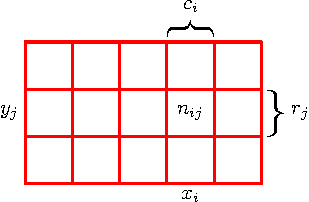
\includegraphics[totalheight=0.4\textheight]{Figure1c10.pdf}
				\caption{Considering in the table $X = x_i$ and $Y = y_j$} }
		\end{figure}
	\end{column}
\end{columns}

\end{frame}

\begin{frame}{\insertsubsection}

Here, we could see some properties that we call \textbf{The Rules of Probability}

\begin{block}{The Rules of Probability}
	\begin{itemize}
		\item Sum Rule: 
		\begin{align} \label{eq:sum-rule}p(X = x_i) =  \sum_j n_{ij} / N
		\visible<2->{ \Rightarrow p(X) = \sum_Y p(X,Y) }
		\end{align}
		\item Product Rule: \begin{align}\label{eq:product-rule}
		p(Y = y_j , X = x_i)=n_{ij}/N \visible<3->{= n_{ij}/c_i \cdot c_i/N}
		\visible<4->{ \Rightarrow p(X,Y) = p(Y|X)p(X) }
\end{align}
\end{itemize}
\end{block}

\end{frame}

\begin{frame}{\insertsubsection}

And by the \textbf{Product Rule} we prove that

\begin{block}{Bayes' Theorem}
\begin{equation}\label{eq:bayes-rule}
	p(X,Y) = p(Y|X)p(X) = p(X|Y)p(Y) \Rightarrow p(Y|X) = \frac{p(X|Y)p(Y)}{p(X)}
\end{equation}
\end{block}

\end{frame}

\begin{frame}{\insertsubsection}

So, from \textbf{The Rules of Probability}, we could show that too 

\begin{block}{Total Probability Theorem}
\begin{equation}\label{eq:total-probability}
	p(X) = \sum_Y p(Y|X)p(X)
\end{equation}
\end{block}

%Remaind of insert the general proof on the appendix

%And so we could derive another formula

%\begin{equation}
%	p(Y|X) = \frac{p(X|Y)p(Y)}{\sum_Y p(Y|X)p(X)}
%\end{equation}

\end{frame}

\begin{frame}{\insertsubsection}

An important propriety of probability is the \textbf{Independence of events}. So, let's say that two events occurs without that one has occurred, so by the \textbf{Bayes' Theorem} we make

\begin{equation}
p(X|Y) = p(X) \text{ and } p(Y|X) = p(Y) \Rightarrow p(X,Y) = p(X)p(Y)
\end{equation}

\end{frame}

\subsection{Random Variables}

\begin{frame}{\insertsubsection}

Simplifying, the \textbf{Random Variables} will treat the probability defined before in the \textit{continuous domain}. So we define a random variable $X$ as a function that assigns a real number, $X(\zeta)$, to each outcome $\zeta$, so $X(\zeta) =  x$.



\end{frame}



\subsection{The Gaussian distribution}
\begin{frame}{\insertsubsection}
The \textbf{Gaussian distribution} is defined as
	\begin{equation}\label{eq:gaussian-distribution}
	\mathcal{N}(x|\mu,\sigma^2) = \frac{1}{(2\pi\sigma^2)^{1/2}}\exp\left\{-\frac{1}{2\sigma^2}(x-\mu)^2\right\}
	\end{equation}
where $\mu$ is the mean and $\sigma^2$ the standard deviation.
\end{frame}


\subsection{Independence of two random variables}
\begin{frame}{\insertsubsection}
\visible<1->{
\begin{block}{Sentence}
\textbf{X and Y are independent random variables} if \textit{any} event $A_1$ defined in terms of $X$ is independent of \textit{any} event $A_2$ defined in terms of Y
\end{block}
}
\visible<2->{
The sentence above is equivalent to say mathematically that
}
\visible<3->{
	\begin{equation}
	P[X \text{ in } A_1, Y \text{ in } A_2]=P[X \text{ in } A_1]P[ Y \text{ in } A_2]
	\end{equation}
}
\visible<4->{
that means in other words that \textit{if $X$ and $Y$ are independent discrete random variables, then the \textbf{joint probability mass function (pmf)} is equal to the product of the marginal pmf's.}
}
\end{frame}

%\begin{frame}{Overleaf users}
%
%\begin{alertblock}{Warning}
%You can ignore this slide if you're \textbf{not} working with Overleaf.
%\end{alertblock}
%
%\vskip 0.5cm
%
%Overleaf, Beamer and Biber do not always get along well together. For this reason, if you make a mistake while writing this presentation, in the drop-down error message you'll \textbf{always} get Biber-related error messages.
%
%\vskip 0.5cm
%
%Luckily, you just have to click on ``\texttt{go to first error/warning}'' and the UI will scroll to the line containing your mistake.
%
%\end{frame}
%
%\begin{frame}[fragile]
%\frametitle{Compiling}
%
%\begin{alertblock}{Warning}
%You can ignore this slide if you're working with Overleaf.
%\end{alertblock}
%
%To compile this deck you'll need the \texttt{biber} package. Probably your \TeX editor already supports it; if not, you will easily find online the instructions to install it.
%
%\vskip 0.5cm
%
%If you're not using an editor, you can compile this presentation using the command line by running:
%
%\begin{verbatim}
%$ pdflatex main.tex
%$ biber main.bcf
%$ pdflatex main.tex
%$ pdflatex main.tex
%\end{verbatim}
%
%
%\end{frame}


\section{Linear Regression}\label{sec:linear-regression}
\framecard{\insertsection}
\subsection{Curve Fitting}

\begin{frame}{\insertsubsection}

\visible<1->{If we have a set of points in the space that comes from observations of an experiment and we want to predict other points, this could be done with \textbf{\textcolor{UniGold}{ curve fitting }}.}

\vspace{0.5em}

\visible<2->{So we could define some strategy to find our model.}

\visible<3->{
	\begin{block}{Strategy}
	\begin{itemize}
		\item[1] Purpose a \textbf{model}, e.g. functions like exponential, polynomial and others.
		\item[2] Train our model with the training data set, finding the \textbf{unknown parameters}.
	\end{itemize}
	\end{block}
}

\end{frame}


\begin{frame}{\insertsubsection}

Let's fit the points below by polynomial curve fitting

	\begin{figure}
	\label{fig:plot-fitting-example}
		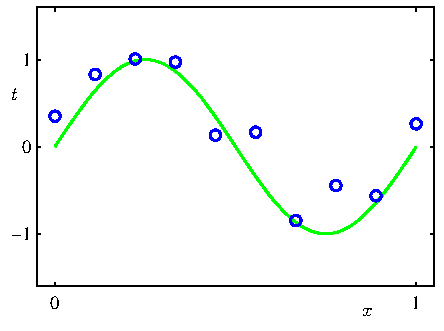
\includegraphics[totalheight=0.75\textheight]{Figure1c2.pdf}
	\end{figure}


\end{frame}

\begin{frame}{\insertsubsection}
Be the model chosen 
\visible<2->{
	\begin{align*}
		y(x,\mathbf{w}) &= w_0x^0 + w_1x^1 + w_2x^2  + ... + w_{M-1}x^{M-1}  = \sum^{M-1}_{j=1} w_j x^j
	\end{align*}
}
\visible<3->{For general, we could write this \textit{weighted sum} with any other function. In other words, we can put this in terms of $\phi_n(x)=x^n$, where $\phi$ could be other \textit{basis function}.
For simplicity, we'll carry this notation along.
}
\visible<4->{
\begin{align*}
	y(x,\mathbf{w}) &= w_0 \phi_0(x) +w_1 \phi_1(x) +w_2 \phi_2(x)  + ... + w_{M-1} \phi_{M-1}(x) = \sum^{M-1}_{j=1} w_j \phi_j(x)
\end{align*}
}
\end{frame}

\begin{frame}{\insertsubsection}

\begin{columns}
\begin{column}{0.45\textwidth}
	\visible<1->{The chosen model will give us some curve that is needed to adjust such that we'll \textit{minimize} his \textbf{distance} to the given points, or \textbf{targets} ($t$).}
	\vspace{0.5em}

	\visible<2->{Here, let's define the sum of these distances as \textit{cost function}, or loss function, and write as}

	\visible<3->{\begin{align*}
	E(\mathbf{w}) \triangleq \frac{1}{2} \sum_{n=1}^N \left\{ y_n -  t_n \right\}^2
	\end{align*}}
\end{column}
\begin{column}{0.475\textwidth}  
    \begin{center}
	\centering
	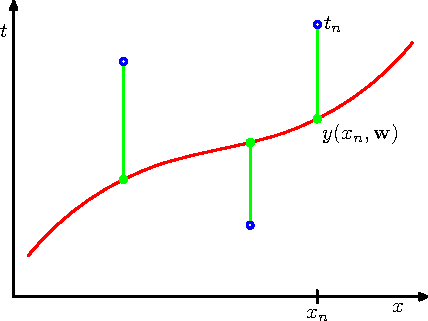
\includegraphics[totalheight=0.55\textheight]{Figure1c3.pdf}
     \end{center}
\end{column}
\end{columns}

\end{frame}
%%%%%%%%%%%%%%%%%%%%%%%%%%%%%%%%%%%
%\begin{frame}{\insertsubsection}

%\textcolor{red}{Insert some \textit{Minkowski} loss.}

%\end{frame}
%%%%%%%%%%%%%%%%%%%%%%%%%%%%%%%%
\begin{frame}{\insertsubsection}
\visible<2->{Remembering that
\begin{align*}
	y_n(x_n,\mathbf{w}) &= w_0 \phi_0(x_n) +w_1 \phi_1(x_n) +w_2 \phi_2(x_n)  + ... + w_{M-1} \phi_{M-1}(x_n)
\end{align*}
%
We could put $y_n(x_i,\mathbf{w})$ in the matricial form and get
%
\begin{equation*}
y_n
=
\begin{bmatrix}
\phi_0(x_n) & \phi_1(x_n) & ... & \phi_{M-1}(x_n)
\end{bmatrix}
\begin{bmatrix}
w_0 \\ w_1 \\  \vdots \\ w_{M-1}
\end{bmatrix}
\end{equation*}}
\end{frame}

\begin{frame}{\insertsubsection}
%
and then
%
\begin{equation*}
\underbrace{
\begin{bmatrix}
y_1 \\ y_2 \\  \vdots \\ y_N
\end{bmatrix}
}_\mathbf{y} = 
\underbrace{
\begin{bmatrix}
\phi_0(x_0) & \phi_1(x_0) & ... & \phi_{M-1}(x_0)   \\ 
\phi_0(x_1) & \phi_1(x_1) & ... & \phi_{M-1}(x_1)    \\ 
\vdots & \vdots & \ddots & \vdots \\
\phi_0(x_{N-1}) & \phi_1(x_{N-1}) & ... & \phi_{M-1}(x_{N-1})  
\end{bmatrix}
}_\Phi
\underbrace{
\begin{bmatrix}
w_1 \\ w_2 \\  \vdots \\ w_N
\end{bmatrix}
}_\mathbf{w}
\end{equation*}
This represents the system $\mathbf{y} = \Phi \mathbf{w}$. If
\begin{align*}
E(\mathbf{w}) =& \frac{1}{2} \left( \mathbf{y} - \mathbf{t} \right)^T\left( \mathbf{y} - \mathbf{t} \right)
\end{align*}
where $\mathbf{t} =
\begin{bmatrix}
t_1 & t_2 & ... & t_n
\end{bmatrix}^T
$
\end{frame}

\begin{frame}{\insertsubsection}
%
Then we'll have 
%
\begin{align*}
E(\mathbf{w}) =& \frac{1}{2} \left( \mathbf{y}^T\mathbf{y} -  \mathbf{t}^T\mathbf{y} - \mathbf{y}^T\mathbf{t} + \mathbf{t}^T\mathbf{t} \right) \\
		   =& \frac{1}{2} \left( ( \Phi \mathbf{w})^T( \Phi \mathbf{w}) -  \mathbf{t}^T( \Phi \mathbf{w}) - ( \Phi \mathbf{w})^T\mathbf{t} + \mathbf{t}^T\mathbf{t} \right) \\
		   =& \frac{1}{2} \left( \mathbf{w}^T \Phi^T \Phi \mathbf{w} -  2\mathbf{t}^T \Phi \mathbf{w} + \mathbf{t}^T\mathbf{t} \right)
\end{align*}
this by the fact that $\alpha =  \mathbf{t}^T( \Phi \mathbf{w}) = ( \Phi \mathbf{w})^T\mathbf{t}$, being $\alpha$ a scalar.

\end{frame}

\begin{frame}{\insertsubsection}
In sequence, we'll try to minimize it in terms of the weights ($\mathbf{w}$) by

\begin{align*}
	0 =& \frac{\partial E(\mathbf{w})}{\partial \mathbf{w}} \\
	0 =& \frac{1}{2} \left( 2 \mathbf{w}^T \Phi^T \Phi  -  2\mathbf{t}^T \Phi + 0 \right) \\
	\mathbf{w}^T =&  \mathbf{t}^T \Phi \left( \Phi^T \Phi \right)^{-1} \\
	\mathbf{w} =& \left( \Phi^T \Phi \right)^{-1}\Phi^T \mathbf{t} \\
\end{align*}

Here, we've obtained $\mathbf{w}$ for the curve fitting.

\end{frame}

\begin{frame}{\insertsubsection}

\begin{figure}
\begin{subfigure}{.3\textwidth}
  \centering
  \includegraphics[width=1\linewidth]{"linear_regression_M1".eps}
\end{subfigure}%
\begin{subfigure}{.3\textwidth}
  \centering
  \includegraphics[width=1\linewidth]{"linear_regression_M2".eps}
\end{subfigure}
\begin{subfigure}{.3\textwidth}
  \centering
  \includegraphics[width=1\linewidth]{"linear_regression_M5".eps}
\end{subfigure}
\begin{subfigure}{.3\textwidth}
  \centering
  \includegraphics[width=1\linewidth]{"linear_regression_M10".eps}
\end{subfigure}%
\begin{subfigure}{.3\textwidth}
  \centering
  \includegraphics[width=1\linewidth]{"linear_regression_M50".eps}
\end{subfigure}
\begin{subfigure}{.3\textwidth}
  \centering
  \includegraphics[width=1\linewidth]{"linear_regression_M100".eps}
\end{subfigure}
\end{figure}

\end{frame}

\begin{frame}{\insertsubsection}

\begin{columns}
\begin{column}{0.45\textwidth}
	\visible<1->{A visible effect of the \textit{increase of the complexity} of the model, represented here by $M$, is the \textit{increase of the weights}. We call it \textbf{over-fitting}.}
	
	\vspace{1em}
	\visible<2->{This phenomenon illustrate a method of ever search for the \textit{best estimation for the parameters}.}
	
	\vspace{1em}
	\visible<3->{It's reasonable to see that our model start's to differ from the $y$ and starts to interpolate the noise.}

	
\end{column}
\begin{column}{0.475\textwidth}  %%<--- here
    \begin{center}
	\centering
	\includegraphics[width=1\linewidth]{"linear_regression_M50".eps}
     \end{center}
\end{column}
\end{columns}

\end{frame}

\begin{frame}{\insertsubsection}

\visible<1->{ To control the over-fitting, we try to \textit{regularize} the weights by adding a penalty term ($\lambda$) to error function, by this we force the coefficients to not reach high values.}

\visible<2->{
		\begin{align*}
			\tilde{E}(\mathbf{w}) =&\frac{1}{2} (\mathbf{y}-\mathbf{t})^T(\mathbf{y}-\mathbf{t}) +\frac{\lambda}{2} \mathbf{w}^T\mathbf{w} \\
		   				    =& \frac{1}{2} \left( \mathbf{w}^T \Phi^T \Phi \mathbf{w} -  2\mathbf{t}^T \Phi \mathbf{w} + \mathbf{t}^T\mathbf{t} + \lambda \mathbf{w}^T\mathbf{I}\mathbf{w} \right) \\
	\Rightarrow \frac{\partial E(\mathbf{w})}{\partial \mathbf{w}} =& \frac{1}{2} \left( 2 \mathbf{w}^T \Phi^T \Phi  -  2\mathbf{t}^T \Phi + 0 + 2 \lambda \mathbf{w}^T \mathbf{I} \right) \\
			0 =&  \mathbf{w}^T \Phi^T \Phi  -  \mathbf{t}^T \Phi + \lambda \mathbf{w}^T \mathbf{I} \\
             \mathbf{w} = & \left( \Phi^T \Phi + \lambda \mathbf{I} \right)^{-1} \Phi^T \mathbf{t}
\end{align*}
}

\end{frame}


%%%%%%%%%%%%%%%%%%%%%%%%%%%%%%%%%%%%%%%%%%%%%%%%%
%
\subsection{A probabilistic perspective}


\begin{frame}{\insertsubsection}
\begin{columns}
\begin{column}{0.45\textwidth}
	\visible<2->{So, we'll start to look the regression with a statistical approach. To encourage you, let's take the sentence.}
	\visible<3->{\vspace{1.5em}
		\begin{block}{Sentence}
		\textit{Having an \textbf{\textcolor{red}{uncertainty}} in the measured value, we could represent it with a  \textbf{\textcolor{red}{probability distribuition}}}.
		\end{block}
   		     }
\end{column}
\begin{column}{0.475\textwidth}  %%<--- here
    \begin{center}
		\visible<4->{
		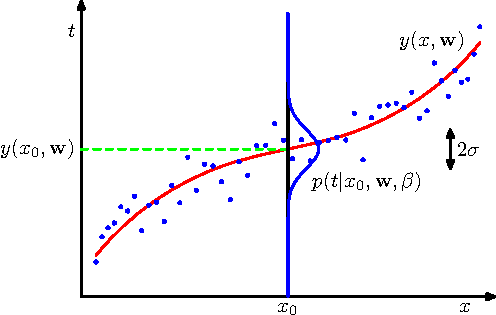
\includegraphics[totalheight=0.5\textheight]{Figure1c16.pdf}
		}
     \end{center}
\end{column}
\end{columns}
\end{frame}

\begin{frame}{\insertsubsection}
\begin{columns}
\begin{column}{0.45\textwidth}
	\visible<1->{Let's go back to the initial problem of curve fitting. Each observation of the phenomenon is described with a random variable whose \textit{mean} is given by $y(x,\mathbf{w})$, and the \textit{variance} by $\beta$. }
	\visible<2->{\vspace{1.5em}\\
			Then, we want to obtain the probability of the \textit{targets}, given some parameters, in this case $\mathbf{x}$, $\mathbf{w}$ and $\beta$.}
\end{column}
\begin{column}{0.475\textwidth}  %%<--- here
    \begin{center}
		\visible<3->{
		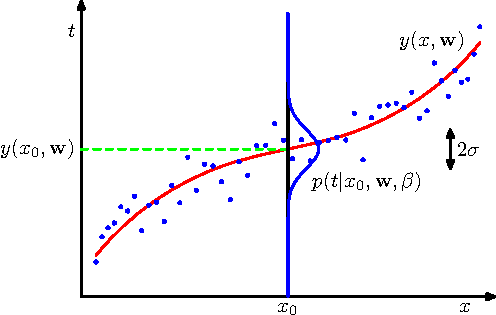
\includegraphics[totalheight=0.5\textheight]{Figure1c16.pdf}
		}
     \end{center}
\end{column}
\end{columns}
\end{frame}

\begin{frame}{\insertsubsection}	
	\visible<1->{So, if we consider that our conditions are such that being the random variables independent and identically distributed, we can say that our \textit{joint probability} is given by
	\begin{equation*}
		p(\mathbf{t} | \mathbf{x}, \mathbf{w}, \beta) = \prod_{n=1}^N p \left( t_n | x_n, \mathbf{w}, \beta \right)
	\end{equation*}
	}
	\visible<2->{Let's assume we have a distribution such that $p( \mathbf{t}| \mathbf{x}, \mathbf{w}, \beta)$. Our goal is, given the \textit{parameters}, maximize the \textit{probability} of the \textit{targets} given the \textit{parameters}. An approach to do this use the fact that
	}
	\visible<2->{
	\begin{equation*}
	\int_\infty ^{-\infty} p(x) dx = 1 \text{ and } p(x) \geq 0
	\end{equation*}}
\end{frame}

\begin{frame}{\insertsubsection}

	Seen this, we're supposing that $p$ could assume values much smaller than one. To avoid computational singularity and for future purposes, we'll take the logarithmic probability. And then
	\begin{equation*}
		\ln \left( p( \mathbf{t}| \mathbf{x}, \mathbf{w}, \beta) \right)
	\end{equation*}
	Reminding that
	\begin{equation*}
		p(\mathbf{t} | \mathbf{x}, \mathbf{w}, \beta) = \prod_{n=1}^N p \left( t_n | x_n, \mathbf{w}, \beta \right)
	\end{equation*}
	Implies that
	\begin{equation*}
		\ln \left( p( \mathbf{t}| \mathbf{x}, \mathbf{w}, \beta) \right) = \sum_{n=1}^N \ln \left(   p \left( t_n | x_n, \mathbf{w}, \beta \right) \right)
	\end{equation*}
\end{frame}

\begin{frame}{\insertsubsection}

\begin{columns}
\begin{column}{0.45\textwidth}
	\visible<1->{To proceed, we need to know what distribution $p$ is. Let's choose the \textbf{\textcolor{UniGold}{Gaussian distribution}}. \\ }
\end{column}
\begin{column}{0.475\textwidth}  %%<--- here
    \begin{center}
		\visible<1->{
		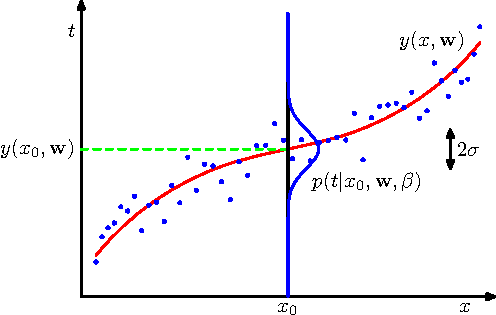
\includegraphics[totalheight=0.5\textheight]{Figure1c16.pdf}
		}
     \end{center}
\end{column}
\end{columns}
\end{frame}

\begin{frame}{\insertsubsection}
\begin{columns}
\begin{column}{0.45\textwidth}

	\visible<1->{The \textbf{\textcolor{UniGold}{Gaussian distribution}} comes from many different contexts, as the one that maximize the entropy among of all ones with fixed variance and from the sum of multiple random variables with finite variance. \\ }
	
\end{column}
\begin{column}{0.475\textwidth}  %%<--- here
    \begin{center}
		\visible<1->{
		\includegraphics[width=1\linewidth]{"Figure1.13".pdf}
		}
     \end{center}
\end{column}
\end{columns}
\end{frame}

\begin{frame}{\insertsubsection}

\begin{block}{One-dimensional Gaussian distribution}
\begin{equation*}
	\mathcal{N}(x | \mu, \sigma^2) = \frac{1}{(2 \pi \sigma^2)^{1/2}} \exp \left\{ -\frac{1}{2 \sigma^2} (x- \mu)^2 \right\} > 0
\end{equation*}
where $\mu$ is the mean and $\sigma^2$ the variance.
\end{block}

\end{frame}

\begin{frame}{\insertsubsection}

Now, back to the discussion of the maximization of 
\begin{equation*}
		\ln \left( p( \mathbf{t}| \mathbf{x}, \mathbf{w}, \beta) \right) = \sum_{n=1}^N \ln \left(   p \left( t_n | x_n, \mathbf{w}, \beta \right) \right)
\end{equation*}

\visible<2->{Reminding that
\begin{equation*}
\mathcal{N}(x | \mu, \sigma^2) = \frac{1}{(2 \pi \sigma^2)^{1/2}} \exp \left\{ -\frac{1}{2 \sigma^2} (x- \mu)^2 \right\}
\end{equation*}
we can state a Gaussian distribution for each target and then
}
\visible<3->{
\begin{equation*}
 p( t| \mathbf{x}, \mathbf{w}, \beta) = \mathcal{N} \left( t | y(\mathbf{x}, \mathbf{w}), \beta^{-1} \right)
\end{equation*}
}

\end{frame}

\begin{frame}{\insertsubsection}
\visible<1->{
And then, from the \textit{joint probability} of the Gaussians distributions

\begin{equation*}
		\ln \left( p( \mathbf{t}| \mathbf{x}, \mathbf{w}, \beta) \right) = \sum_{n=1}^N - \frac{1}{2} \ln (2 \pi) + \sum_{n=1}^N \frac{1}{2} \ln \beta - \sum_{n=1}^N \frac{\beta}{2} (x_n -  y(x_n, \mathbf{w}))^2
\end{equation*}
}
\visible<2->{From this, we could obtain the \textbf{maximum likelihood}, or the \textit{best estimation for the parameters}, taking the derivatives of the log probability to zero, according to the terms $\beta$ and $\mathbf{w}$, our model parameters. We'll obtain
\begin{equation*}
\frac{1}{\beta_{ML}} = \frac{1}{N} \sum^N_{n=1} \left\{ y(x_n, \mathbf{w}_{ML}) - t_n \right\}^2
\end{equation*}
remembering that $\mathbf{w}_{ML}$ is already known from the regular linear regression.
}
%Maximizing with respect to $\beta$, we'll have 

%\begin{equation*}
%		\frac{1}{\beta_{ML}} = \frac{1}{N} \sum^N_{n=1} \left\{ y(x_n, \mathbf{w}_{ML}) - t_n \right\}^2
%\end{equation*}
%
%where $\beta_{ML}$ is the precision parameter for the maximum likelihood for the conditional Gaussian distribution.
\end{frame}

\begin{frame}{\insertsubsection}
We could observe that taking the derivative with respect to $\mathbf{w}$, our expression becomes closer to the \textit{error function} presented previously, added the dependency of $\beta$

\begin{align*}
	E(\mathbf{w}) \triangleq \frac{1}{2} \sum_{n=1}^N \left\{ y_n -  t_n \right\}^2
\end{align*}

Then some behaviors could be expected, as the \textbf{over-fitting}.

%Maximizing with respect to $\beta$, we'll have 

%\begin{equation*}
%		\frac{1}{\beta_{ML}} = \frac{1}{N} \sum^N_{n=1} \left\{ y(x_n, \mathbf{w}_{ML}) - t_n \right\}^2
%\end{equation*}
%
%where $\beta_{ML}$ is the precision parameter for the maximum likelihood for the conditional Gaussian distribution.
\end{frame}

\begin{frame}{\insertsubsection}

At this point, we have a probabilistic model and we may want to predict values for $x$. Then, we need a \textit{predictive distribution}. \\
\vspace{1em}
Let's say we have the probabilities of some idea we desire to update it in the light of some new evidence. This could be done with \textbf{Bayes' Theorem}, to convert a \textit{prior} probability in a \textit{posterior} probability. \\
\end{frame}

\begin{frame}{\insertsubsection}
Mathematically, by Bayes' Theorem and the \textbf{Product Rule}, we could infer
\visible<2->{
\begin{equation*}
p\left( \mathbf{w} | \mathbf{x}, \mathbf{t}, \alpha, \beta \right) \propto p\left(  \mathbf{t} |\mathbf{w} ,\mathbf{x}, \beta \right)  p\left( \mathbf{w} | \alpha \right)
\end{equation*}
}
\visible<3->{
and by simplicity, consider
\begin{equation*}
p \left( \mathbf{w} | \alpha \right) = \mathcal{N} \left( \mathbf{w} | \boldsymbol{0}, \alpha^{-1} \mathbf{I} \right) = \left(  \frac{\alpha}{2 \pi}\right) ^{(M+1)/2} \exp \left\{ - \frac{\alpha}{2} \mathbf{w}^T \mathbf{w} \right\}
\end{equation*}
where $\alpha$ is the precision of the distribution ans $M+1$ is the dimension of $\mathbf{w}$, for a polynomial of $M^{th}$ order.
}
\end{frame}

\begin{frame}{\insertsubsection}
By this, we can find a distribution and its maximum, or most probable value of $\mathbf{w}$ given the data taking the minimum of the negative logarithm of the infered expression, that wll lead us to a term

\begin{equation*}
\sum^N_{n=1} \left\{ y(x_n, \mathbf{w}) - t_n \right\}^2 + \frac{\alpha}{2} \mathbf{w}^T\mathbf{w}
\end{equation*}

Note that if we consider $\lambda = \alpha / \beta$, this will back to the regularized form of \textit{least squares}.
\end{frame}

\begin{frame}{\insertsubsection}

So, observe that, even making some probabilistic assumptions, we don't have yet a fully bayesian model, given that finding the \textit{maximum likelihood}, we're finding only the parameters given one model such that maximize our targets probabilities. Furthermore, even with some probabilistic assumptions, our model still have a \textbf{over-fitting} problem, given that we obtained the same expressions.\\
\vspace{1em}
The next step is put some \textbf{uncertainty in predictive model}, and makes adjustments in the light of our new evidences. By that we could obtain a "more Bayesian" model, in other words, a \textcolor{UniGold}{\textbf{Bayesian Linear Regression}}.

\end{frame}

%\begin{frame}{\insertsubsection}
%	\visible<1->{Let's take a look at the Bayes Theorem}
%	
%	\visible<2->{
%	\begin{block}{Bayes Theorem}{
%			\begin{equation*}\label{bayes_theorem}
%				\visible<2->{ p(\mathbf{w}|\mathcal{D}) = \frac{p(\mathcal{D}| \mathbf{w}) p(\mathbf{w}) } {  p(\mathcal{D}) } } 
%			\end{equation*}
%			}
%	\end{block}
%	\visible<3->{The new role of Bayes Theorem here is the fact that we could obtain new, or better, probability distribuitions for the weights in light of an determined data set $\mathcal{D}$.}
%	}
%\end{frame}

%\begin{frame}{\insertsubsection}
%	\visible<1->{\textbf{\textcolor{UniGold}{At this time, it's important to point out some things. \\}}}
%	\vspace{1.5em}
%	\visible<2->{When we write $ p \left( t_n | x_n, \mathbf{w}, \beta \right)$, we assume a probability distribuition over the parameters $\mathbf{w}$ and $\beta$ too.\\}
%	\vspace{1.5em}
%	\visible<3->{Then we could observe that we'll obtain a \textbf{discrete distribution of functions} in their \textit{parameters}.\\}
%	\vspace{1.5em}
%	\visible<4->{So, here is where the Bayes Theorem plays an important role by \textbf{adjusting} these \textit{parameters} as we obtain evidences.}
%\end{frame}
%
%\begin{frame}{\insertsubsection}
%	\visible<1->{Taking some steps back, let's re-visit the \textbf{Curve Fitting}. There, the strategy was minimize the error function.\vspace{1.5em} \\}
%	\visible<2->{Now we'll try to view the same problem with a \textit{probabilistic perspective}. We're trying to make predictions for the target value $\mathbf{t}$ given some new values of $x$.\vspace{1.5em} \\}
%
%\end{frame}


%\begin{frame}{\insertsubsection}
%	And taking the derivatives with respect to $\beta$ to minimize the error	
%		\begin{align*}
%		\visible<1->{
%			\frac{\partial}{\partial \beta}\ln \left( p( \mathbf{t}| \mathbf{x}, \mathbf{w}, \beta) \right) &=0 } \\
%		\visible<2->{
%			 -\frac{1}{2} \sum^N_{n=1} \left\{ y(x_n,\mathbf{w} -t_n ) \right\}^2 + \frac{N}{2}\frac{1}{\beta} &= 0 \\  }
%		\visible<3->{
%			 \frac{1}{N} \sum^N_{n=1} \left\{ y(x_n,\mathbf{w} -t_n ) \right\}^2  &= \frac{1}{\beta_{ML}}  }
%		\end{align*}
%	\visible<4->{
%	Where $\beta_{ML}$ is the maximum likelihood.}
%
%\end{frame}

\section{Bayesian Linear Regression}

\framecard{\insertsection}

\begin{frame}{\insertsection}
	\framesubtitle{Bayesian vs. Frequentist statistics}
	
	\textcolor{UniGold}{\textbf{What if we assume not knowing the data exactly?}}

	\begin{columns}
		\begin{column}{0.475\textwidth}
			\begin{itemize}
				\item The principle of the Bayesian statistics is express our \textcolor{UniOrange}{\textbf{degree of belief}} in an event.
				\item This belief could be based on some \textcolor{UniOrange}{\textbf{prior}} knowledge about the event or personal beliefs.
				\item This differs from frequentist statistics, where the probability is based on the number of trials.
				\item Suppose a die to be thrown once
			\end{itemize}
			\only<1>{
			\begin{block}{Frequentist}
				There's empiric evidence that similar dice thrown in past produce similar outcomes with the same frequency.
			\end{block}}
			\only<2>{
			\begin{exampleblock}{Bayesian}
				The last argument is right, but the \textcolor{UniBlue}{\textbf{belief of the observer}} it's important to the statistics, as the number of the Lotto.
			\end{exampleblock}}
			\end{column}
			\begin{column}{0.475\textwidth}   
				\centering
				\begin{figure}
					\includegraphics[width=1\linewidth]{"Triplot-of-prior-likelihood-and-posterior"}
				\caption{\cite{AksuAnil2018}}
				\end{figure}
			\end{column}
		\end{columns}
\end{frame}
	
\begin{frame}{\insertsection}
	\framesubtitle{Bayes' Rule}

	\begin{itemize}
		\item The main idea of the Bayesian approach is put some \textcolor{UniOrange}{\textbf{uncertainty}} over the parameters and make \textcolor{UniOrange}{\textbf{inferences}}, i.e. obtain some statistics in light over the data.
		\item This principle is elucidated by the Bayes' Rule
		\begin{equation*}
			\overbrace{p(\mathbf{w}|\mathbf{t})}^{posterior} = \frac{p(\mathbf{t}|\mathbf{w}) p(\mathbf{w})}{p(\mathbf{t})} = \frac{\overbrace{p(\mathbf{t}|\mathbf{w})}^{\text{\textit{likelihood}}} \overbrace{p(\mathbf{w})}^{\text{\textit{prior}}}}{\underbrace{\int p(\mathbf{t}|\mathbf{w}) p(\mathbf{w}) d\mathbf{w}}_{\text{\textit{marginal distribution}}}}
		 \end{equation*}
		 where we assume some uncertainty over the parameters, i.e. a probability density function $p(\mathbf{w})$.
		 \item We'll use the knowledge about the data with the \textcolor{UniOrange}{\textbf{likelihood function}} and some previous knowledge, or \textcolor{UniOrange}{\textbf{prior}}, that we have about the parameters to obtain the knowledge considering these two, or \textcolor{UniOrange}{\textbf{posterior}}.
		 \item This is called \textcolor{UniOrange}{\textbf{Bayesian Inference}}.
	\end{itemize}
% \visible<2->{
% \begin{equation*}
% \underbrace{p\left( \mathbf{w} | \mathbf{x}, \mathbf{t}, \alpha, \beta \right)}_{\text{posterior}} \propto \underbrace{p\left(  \mathbf{t} |\mathbf{w} ,\mathbf{x}, \beta \right)}_{\text{likelihood}}  \underbrace{p\left( \mathbf{w} | \alpha \right)}_{\text{prior}}
% \end{equation*}
% }
% \visible<3->{
% and for simplicity, consider the follow prior for $\mathbf{w}$
% \begin{equation*}
% p \left( \mathbf{w} | \alpha \right) = \mathcal{N} \left( \mathbf{w} | \boldsymbol{0}, \alpha^{-1} \mathbf{I} \right) = \left(  \frac{\alpha}{2 \pi}\right) ^{(M+1)/2} \exp \left\{ - \frac{\alpha}{2} \mathbf{w}^{\top} \mathbf{w} \right\}
% \end{equation*}
% where $\alpha$ the precision of the distribution and $M+1$ is the dimension of $\mathbf{w}$, for a polynomial of $M^{th}$ order. Variables such $\alpha$ are called \textit{hyperparameters} and control the distribuition of model parameters.}
\end{frame}

\begin{frame}{\insertsubsection}
By this, we can find a distribution and its maximum, or most probable value of $\mathbf{w}$ given the data taking the minimum of the negative logarithm of the infered expression, that will lead us to a term

\begin{equation*}
\sum^N_{n=1} \left\{ y(x_n, \mathbf{w}) - t_n \right\}^2 + \frac{\alpha}{2} \mathbf{w}^{\top}\mathbf{w} + \text{const.}
\end{equation*}

Note that if we consider $\lambda = \alpha / \beta$, this will back to the regularized form of \textit{least squares}. This technique is called \textit{maximum posterior} (MAP).
\end{frame}

\begin{frame}{\insertsubsection}

So, observe that even making some probabilistic assumptions, we don't have yet a fully bayesian model, given that finding the \textit{maximum likelihood}, we're finding only the parameters given one model such that maximize our targets probabilities. Furthermore, even with some probabilistic assumptions, our model still have a \textbf{over-fitting} problem, given that we obtained the same expressions for the simple regression, adding some constants.\\
\vspace{1em}
The next step is put some \textbf{uncertainty in predictive model}, and makes adjustments in the light of our new evidences. By that we could obtain a "more Bayesian" model, in other words, a \textcolor{UniGold}{\textbf{Bayesian Linear Regression}}.

\end{frame}

%\begin{frame}{\insertsubsection}
%	\visible<1->{Let's take a look at the Bayes Theorem}
%	
%	\visible<2->{
%	\begin{block}{Bayes Theorem}{
%			\begin{equation*}\label{bayes_theorem}
%				\visible<2->{ p(\mathbf{w}|\mathcal{D}) = \frac{p(\mathcal{D}| \mathbf{w}) p(\mathbf{w}) } {  p(\mathcal{D}) } } 
%			\end{equation*}
%			}
%	\end{block}
%	\visible<3->{The new role of Bayes Theorem here is the fact that we could obtain new, or better, probability distribuitions for the weights in light of an determined data set $\mathcal{D}$.}
%	}
%\end{frame}

%\begin{frame}{\insertsubsection}
%	\visible<1->{\textbf{\textcolor{UniGold}{At this time, it's important to point out some things. \\}}}
%	\vspace{1.5em}
%	\visible<2->{When we write $ p \left( t_n | x_n, \mathbf{w}, \beta \right)$, we assume a probability distribuition over the parameters $\mathbf{w}$ and $\beta$ too.\\}
%	\vspace{1.5em}
%	\visible<3->{Then we could observe that we'll obtain a \textbf{discrete distribution of functions} in their \textit{parameters}.\\}
%	\vspace{1.5em}
%	\visible<4->{So, here is where the Bayes Theorem plays an important role by \textbf{adjusting} these \textit{parameters} as we obtain evidences.}
%\end{frame}
%
%\begin{frame}{\insertsubsection}
%	\visible<1->{Taking some steps back, let's re-visit the \textbf{Curve Fitting}. There, the strategy was minimize the error function.\vspace{1.5em} \\}
%	\visible<2->{Now we'll try to view the same problem with a \textit{probabilistic perspective}. We're trying to make predictions for the target value $\mathbf{t}$ given some new values of $x$.\vspace{1.5em} \\}
%
%\end{frame}


%\begin{frame}{\insertsubsection}
%	And taking the derivatives with respect to $\beta$ to minimize the error	
%		\begin{align*}
%		\visible<1->{
%			\frac{\partial}{\partial \beta}\ln \left( p( \mathbf{t}| \mathbf{x}, \mathbf{w}, \beta) \right) &=0 } \\
%		\visible<2->{
%			 -\frac{1}{2} \sum^N_{n=1} \left\{ y(x_n,\mathbf{w} -t_n ) \right\}^2 + \frac{N}{2}\frac{1}{\beta} &= 0 \\  }
%		\visible<3->{
%			 \frac{1}{N} \sum^N_{n=1} \left\{ y(x_n,\mathbf{w} -t_n ) \right\}^2  &= \frac{1}{\beta_{ML}}  }
%		\end{align*}
%	\visible<4->{
%	Where $\beta_{ML}$ is the maximum likelihood.}
%
%\end{frame}

\begin{frame}{\insertsection}
	Seeking a Bayesian approach, the next steps consists to apply the \textbf{sum} and \textbf{product} rules of probability to evaluate the predictive distribution. By now we assume that the hyperparameters are fixed, but they could assume a distribution too. \\
	\vspace{1em}
	We saw that the posterior distribution for $\mathbf{w}$ could be given by
	\begin{equation*}
		\underbrace{p\left( \mathbf{w} | \mathbf{x}, \mathbf{t} \right)}_{\text{posterior}} \propto \underbrace{p\left(  \mathbf{t} |\mathbf{w} ,\mathbf{x} \right)}_{\text{likelihood}}  \underbrace{p\left( \mathbf{w} \right)}_{\text{prior}}
	\end{equation*}

\end{frame}


\subsection{The D-dimensional Gaussian Distribution}

\begin{frame}{\insertsubsection}

Remember the One-dimensional Gaussian distribution
\begin{block}{One-dimensional Gaussian distribution}
\begin{equation*}
	\mathcal{N}(x | \mu, \sigma^2) = \frac{1}{(2 \pi \sigma^2)^{1/2}} \exp \left\{ -\frac{1}{2 \sigma^2} (x- \mu)^2 \right\} > 0
\end{equation*}
where $\mu$ is the mean and $\sigma^2$ the variance.
\end{block}
\visible<2->{\vspace{1em}
			First we'll consider a geometrical approach by the quadratic distance $(x -  \mu)^2$ normalized by the variance $\sigma^2$. This comprehension will help us with the D-dimensional case.
   		     	}
\end{frame}

\begin{frame}{\insertsubsection}
	To more than one dimensions, we'll consider the points ($x$) distance for the mean of the distribution, as we done in the one dimensional case, by adding a term to prioritize some dimension distribution in particular. Then
	\begin{equation*}
		\Delta^2 = (\mathbf{x} - \boldsymbol{\mu})^{\top} \boldsymbol{\Sigma} ^{-1} (\mathbf{x} - \boldsymbol{\mu}) 
	\end{equation*}
called \textit{Mahalanobis distance}. And it's becomes the \textit{Euclidean distance}, when $\boldsymbol{\Sigma}$ is the indentity matrix. This means that the all the distances are equally normalized. The matrix $\boldsymbol{\Sigma}$ is the covariance matrix of the distributions, by definition.
\end{frame}

\begin{frame}{\insertsubsection}
And then
\begin{block}{D-dimensional Gaussian distribution}
\begin{equation*}
	\mathcal{N}(\mathbf{x} | \boldsymbol{\mu}, \boldsymbol{\Sigma}) = \frac{1}{(2 \pi )^{D/2}} \frac{1}{|\boldsymbol{\Sigma}|^{1/2}} \exp \left\{ -\frac{1}{2} (\mathbf{x} - \boldsymbol{\mu})^{\top} \boldsymbol{\Sigma} ^{-1} (\mathbf{x} - \boldsymbol{\mu})  \right\} 
\end{equation*}
where $\boldsymbol{\mu}$ is the D-dimensional mean vector, $\boldsymbol{\Sigma}$ the D$\times$D-dimensional variance matrix and $|\boldsymbol{\Sigma}|$ its determinant.
\end{block}
\end{frame}

 \begin{frame}{\insertsubsection}
 
 \begin{block}{Partitioned Gaussians}
 Given a joint Gaussian distribution $\mathcal{N}(\mathbf{x} | \boldsymbol{\mu}, \boldsymbol{\Sigma})$ with $\boldsymbol{\Lambda} \equiv \boldsymbol{\Sigma}^{-1}$ and
 \begin{equation*}
 	\mathbf{x} = 
 	 \begin{pmatrix}
 		\mathbf{x} _{a} \\
 		\mathbf{x} _{b}
 	\end{pmatrix} , 
 	\boldsymbol{\mu} = 
 	 \begin{pmatrix}
 		\boldsymbol{\mu}_{a} \\
 		\boldsymbol{\mu}_{b}
 	\end{pmatrix} , 
 	 \boldsymbol{\Sigma} = 
 	 \begin{pmatrix}
 		\boldsymbol{\Sigma}_{aa} & \boldsymbol{\Sigma}_{ab} \\
 		\boldsymbol{\Sigma}_{ba} & \boldsymbol{\Sigma}_{bb} 
 	\end{pmatrix} ,  \boldsymbol{\Lambda} = 
 	 \begin{pmatrix}
 		\boldsymbol{\Lambda}_{aa} & \boldsymbol{\Lambda}_{ab} \\
 		\boldsymbol{\Lambda}_{ba} & \boldsymbol{\Lambda}_{bb} 
 	\end{pmatrix}.
 \end{equation*}
 Will give us \\
 \begin{itemize}
 \item \textcolor{UniGold}{Conditional distribution:}
 \begin{equation*}
 p\left( \mathbf{x}_a | \mathbf{x}_b \right) = \mathcal{N}\left( \mathbf{x}_a| \boldsymbol{\mu}_{a|b}, \boldsymbol{\Lambda}^{-1}_{aa} \right), \  \boldsymbol{\mu}_{a|b} =  \boldsymbol{\mu}_a - \boldsymbol{\Lambda}^{-1}_{aa}\boldsymbol{\Lambda}_{ab} \left( \mathbf{x}_b - \boldsymbol{\mu}_b \right)
 \end{equation*}

 \item \textcolor{UniGold}{Marginal distribution:}
 \begin{equation*}
 p\left( \mathbf{x}_a \right) = \mathcal{N} \left( \mathbf{x}_a | \boldsymbol{\mu}_a,\boldsymbol{\Sigma}_{aa} \right)
 \end{equation*}
 \end{itemize}

 \end{block}
 \end{frame}


\subsection{Bayes' rule for Gaussian variables}

\begin{frame}{\insertsubsection}

To proceed we'd like to prove that the Gaussians are \textbf{closed under linear transformations}. This will allow us to transform the Gaussians under the likelihood distribution given a prior. For example, given a distribution

\begin{equation*}
	p(\mathbf{z}) = p(\mathbf{x},\mathbf{y})
\end{equation*}

\end{frame}

\begin{frame}{\insertsubsection}
\visible<1->{
	In other words, we're trying to find the parginal distribution $p\left( \mathbf{y} \right)$ and the conditional distribution $p\left( \mathbf{x} | \mathbf{y} \right)$, given
	\begin{align*}
	p\left( \mathbf{x} \right) =& \mathcal{N} \left( \mathbf{x}|\boldsymbol{\mu}, \boldsymbol{\Lambda}^{-1} \right) \\
	p\left( \mathbf{y} | \mathbf{x} \right) =& \mathcal{N} \left( \mathbf{y}|\mathbf{Ax}+\mathbf{b}, \mathbf{L}^{-1} \right)
	\end{align*}
}
\visible<2->{
So, applying the joint distribution and the its $\ln$ after
	\begin{align*}
	p\left( \mathbf{z} \right) =& \ p\left(  \mathbf{x}, \mathbf{y} \right) = p\left(  \mathbf{y} | \mathbf{x} \right) p\left( \mathbf{x} \right) \\
	\ln p\left( \mathbf{z} \right) =& \ln p\left(  \mathbf{y} | \mathbf{x} \right) + \ln p\left( \mathbf{x} \right)  \\
					   =&  -\frac{1}{2}\left( \mathbf{x} - \boldsymbol{\mu} \right)^{\top}\boldsymbol{\Lambda}\left( \mathbf{x} - \boldsymbol{\mu} \right) \\ & -\frac{1}{2} \left( \mathbf{y} - \mathbf{Ax} - \mathbf{b} \right)^{\top} \mathbf{L} \left( \mathbf{y} - \mathbf{Ax} - \mathbf{b} \right)+ \text{const}
	\end{align*}
}
\end{frame}

\begin{frame}{\insertsubsection}
\visible<1->{
	The "const" is the term independent of $\mathbf{x}$ and $\mathbf{y}$. Then, expanding the quadratic form
	\begin{align*}
	\ln p\left( \mathbf{z} \right) =&  -\frac{1}{2} \mathbf{x}^{\top} \left( \boldsymbol{\Lambda} + \mathbf{A}^{\top} \mathbf{L} \mathbf{A} \right) \mathbf{x} - \frac{1}{2} \mathbf{y}^{\top} \mathbf{Ly} + \frac{1}{2} \mathbf{y}^{\top} \mathbf{LAx} + \frac{1}{2} \mathbf{x}^{\top} \mathbf{A}^{\top} \mathbf{Ly} \\ 
					   =& - \frac{1}{2} \begin{pmatrix} \mathbf{x} \\ \mathbf{y} \end{pmatrix}^{\top} \begin{pmatrix} \boldsymbol{\Lambda} + \mathbf{A}^{\top} \mathbf{LA} & -\mathbf{A}^{\top} \mathbf{L} \\ -\mathbf{LA} & \mathbf{L} \end{pmatrix}  \begin{pmatrix} \mathbf{x} \\ \mathbf{y} \end{pmatrix} = - \frac{1}{2} \mathbf{z}^{\top} \mathbf{Rz}
	\end{align*}
}
\visible<2->{
	We'll apply the partitioned matrices inversion to obtain $\mathbf{R}^{-1}$
	\begin{align*}
	\mathbf{R}^{-1} =& \begin{pmatrix} \boldsymbol{\Lambda}^{-1} & \boldsymbol{\Lambda}^{-1}\mathbf{A}^{\top} \\ \mathbf{A}\boldsymbol{\Lambda}^{-1} & \mathbf{L}^{-1} + \mathbf{A}\boldsymbol{\Lambda}^{-1}\mathbf{A}^{\top} \end{pmatrix}
	\end{align*}
}
\end{frame}

\begin{frame}{\insertsubsection}
\visible<1->{
	The expanded form of $\ln p\left( \mathbf{z} \right)$ give us the mean too by the linear terms, then
	\begin{align*}
	\mathbf{x}^{\top} \boldsymbol{\Lambda \mu}  -\mathbf{x}^{\top} \mathbf{A}^{\top} \mathbf{Lb} + \mathbf{y}^{\top} \mathbf{Lb} = \begin{pmatrix} \mathbf{x} \\ \mathbf{y} \end{pmatrix}^{\top} \begin{pmatrix} \boldsymbol{\Lambda \mu} - \mathbf{A}^{\top} \mathbf{Lb} \\ \mathbf{Lb}  \end{pmatrix}
	\end{align*}
}
\visible<2->{
	By inspection of the linear terms
	\begin{align*}
	\mathbb{E}[\mathbf{z}] = \mathbf{R}^{-1} \begin{pmatrix} \boldsymbol{\Lambda \mu} - \mathbf{A}^{\top} \mathbf{Lb} \\ \mathbf{Lb}  \end{pmatrix} =  \begin{pmatrix} \boldsymbol{\mu}  \\  \mathbf{A}\boldsymbol{\mu} + \mathbf{b}  \end{pmatrix}
	\end{align*}
}
\end{frame}

\begin{frame}{\insertsubsection}
And then we we'll have that
\visible<1->{
	\begin{align*}
	\mathbb{E}[\mathbf{y}] =& \ \mathbf{A}\boldsymbol{\mu} + \mathbf{b} \\
	\text{cov}[\mathbf{y}] =& \ \mathbf{L}^{-1} + \mathbf{A}\boldsymbol{\Lambda}^{-1}\mathbf{A}^{\top}
	\end{align*}
}
\visible<2->{
	\begin{align*}
	\mathbb{E}[\mathbf{x}|\mathbf{y}] =& \ \left(  \boldsymbol{\Lambda} + \mathbf{A}^{\top} \mathbf{LA} \right)^{-1} \left\{ \mathbf{A}^{\top} \mathbf{L}(\mathbf{y}- \mathbf{b}) + \boldsymbol{\Lambda \mu} \right\} \\
	\text{cov}[\mathbf{x}|\mathbf{y}] =& \ \left(  \boldsymbol{\Lambda} + \mathbf{A}^{\top} \mathbf{LA} \right)^{-1}
	\end{align*}
}
\end{frame}

\begin{frame}{\insertsection}
In the next step, we'll assume a \textbf{prior distribution over parameters}, $p(\mathbf{w})$, and define it as a Gaussian distribution, then
\begin{equation*}
	p(\mathbf{w}) = \mathcal{N} \left( \mathbf{w} | \mathbf{m}_0, \mathbf{S}_0 \right)
\end{equation*}	
with mean $\mathbf{m}_0$ and variance $\mathbf{S}_0$.
\end{frame}


%%%%%%%%%%%%%%%%%%%%%%%%%%%%%%%%%%%%%%%%%%%%%%%%%%%%%%%%%%%%%%%%%%%%

\begin{frame}{\insertsubsection}

\begin{block}{Marginal and Conditioned Gaussians}

\begin{itemize}
\item \textcolor{UniGold}{For $\mathbf{y}$ given $\mathbf{x}$:}
\begin{align*}
	p\left( \mathbf{x} \right) =& \mathcal{N} \left( \mathbf{x}|\boldsymbol{\mu}, \boldsymbol{\Lambda}^{-1} \right) \\
	p\left( \mathbf{y} | \mathbf{x} \right) =& \mathcal{N} \left( \mathbf{y}|\mathbf{Ax}+\mathbf{b}, \mathbf{L}^{-1} \right)
\end{align*}

\item \textcolor{UniGold}{For $\mathbf{x}$ given $\mathbf{y}$:}
\begin{align*}
p\left( \mathbf{x} | \mathbf{y} \right) =& \ \mathcal{N}\left( \mathbf{y}| ,  \boldsymbol{\Sigma} \left\{ \mathbf{A}^{\top} \mathbf{L}(\mathbf{y}-\mathbf{b} + \boldsymbol{\Sigma \mu}) \right\}, \boldsymbol{\Sigma} \right) \\
p\left( \mathbf{y} \right) =& \ \mathcal{N}\left( \mathbf{y}|\mathbf{A} \boldsymbol{\mu} + \mathbf{b}, \mathbf{L}^{-1} + \mathbf{A}\boldsymbol{\Lambda}^{-1}\mathbf{A}^{\top} \right) \text{, where } \boldsymbol{\Sigma} = \left(  \boldsymbol{\Lambda} + \mathbf{A}^{\top} \mathbf{LA} \right)^{-1}
\end{align*}
\end{itemize}

\end{block}
\end{frame}

\begin{frame}{\insertsubsection}
	By the derivations, we make the assumptions of given $p(\mathbf{w})$ and  for $p(\mathbf{t}|\mathbf{w})$ such that 
	\begin{align*}
		p(\mathbf{t}|\mathbf{w}) &= \mathcal{N}\left( \mathbf{t}|y(\mathbf{x},\mathbf{w}), \beta^{-1} \right)	\\
		&= \mathcal{N}\left( \mathbf{t}|\boldsymbol{\Phi}^{\top}\mathbf{w}, \beta^{-1} \right)
	\end{align*}
	And then $p(\mathbf{w}|\mathbf{t}) = \mathcal{N}\left( \mathbf{w}|\mathbf{m}_N, \mathbf{S}_N \right)$ where
	\begin{align*}
		\mathbf{m}_N &= \mathbf{S}_N \left( \mathbf{S}_0^{-1}\mathbf{m}_0 + \beta \boldsymbol{\Phi}^{\top}\mathbf{t}  \right) \\
		\mathbf{S}_N^{-1} &= \mathbf{S}_0^{-1} + \beta\boldsymbol{\Phi}^{\top}\boldsymbol{\Phi}
	\end{align*}
\end{frame}

% \begin{frame}{\insertsubsection}
% 	We'll make the same optimization we made for the mono-variate case. So the logarithmic likelihood results 
% 	\begin{block}{Maximum likelihood for the Gaussian}
% 	\begin{equation*}
% 	\ln p \left( \mathbf{X} | \boldsymbol{\mu}, \boldsymbol{\Sigma} \right) =
% 	- \frac{N D}{2} \ln (2 \pi) - \frac{N}{2} \ln |\boldsymbol{\Sigma}| - 
% 	\frac{1}{2} \sum^N_{n=1} \left( \mathbf{x}_n - \boldsymbol{\mu} \right)^{\top} 
% 	\Sigma^{-1} \left( \mathbf{x}_n - \boldsymbol{\mu} \right)
% 	\end{equation*}	
% 	\end{block}

% \end{frame}
%%%%%%%%%%%%%%%%%%%%%%%%%%%%%%%%%%%%%%%%%%%%

\section{Gaussian Processes}
\framecard{\insertsection}

% \subsection{Recap}
% \begin{frame}{\insertsubsection}
%     \framesubtitle{Linear Regression} 

%     \textcolor{UniGold}{\textbf{What was done until here?}}
%     \begin{itemize}
%         \item We assumed that our targets $t$ were \textcolor{UniOrange}{\textbf{i.i.d.}} and given by $t = y(\mathbf{x}) + \varepsilon$, where $\varepsilon \sim \mathcal{N}(0,\beta)$.
%         \item Our model is given by $\mathbf{y}(\mathbf{x}) = \Phi^{\top} \mathbf{w}$, where $\Phi$ is the \textcolor{UniOrange}{\textbf{design matrix}}, and this caracterize our model as \textcolor{UniOrange}{\textbf{linear in parameters}}.
%         \item The \textcolor{UniOrange}{\textbf{design matrix}} was defined as $ \phi_{i,j} = \phi_i(\mathbf{x}_j)$.
%         \item The \textcolor{UniOrange}{\textbf{parameters}} were given by $\mathbf{w} = \left( \Phi^{\top} \Phi \right)^{-1}\Phi^{\top} \mathbf{t}$.
%         \item These \textcolor{UniOrange}{\textbf{parameters}} calculated at the minimum of the cost function are called \textcolor{UniOrange}{\textbf{maximum likelihood}}.
%     \end{itemize}
%     \begin{columns}
%         \begin{column}{0.5\linewidth}  
%         \begin{center}
%         \centering
%         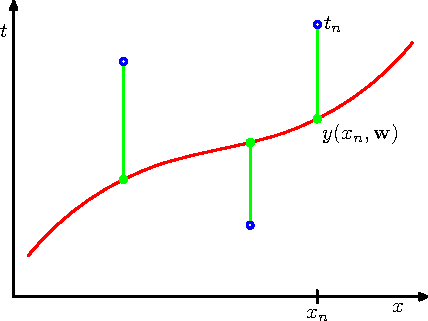
\includegraphics[width=0.9\linewidth]{Figure1c3.pdf}
%          \end{center}
%     \end{column}
%     \begin{column}{0.5\linewidth}  %%<--- here
%         \begin{figure}
%             \setlength\fwidth{0.07\textwidth}
%             \input{./codes/lnReg/"lnReg".tex}
%         \end{figure}
%     \end{column}
%     \end{columns}

% \end{frame}

% \begin{frame}{\insertsubsection}
%     \framesubtitle{Bayesian Linear Regression} 

%     \textcolor{UniGold}{\textbf{What was done until here?}}
%     \begin{itemize}
%         \item We put an \textcolor{UniOrange}{\textbf{uncertainty}} over the targets $t$ and the parameters $\mathbf{w}$.
%         \item We assumed that targets being \textcolor{UniOrange}{\textbf{distributed}} as $p( t| \mathbf{x}, \mathbf{w}, \beta) = \mathcal{N} ( t | y(\mathbf{x}, \mathbf{w}), \beta^{-1})$.
%         \item By \textcolor{UniOrange}{\textbf{Bayes' Rule}} we obtained that $p\left( \mathbf{w} | \mathbf{x}, \mathbf{t}, \alpha, \beta \right) \propto p\left(  \mathbf{t} |\mathbf{w} ,\mathbf{x}, \beta \right) p\left( \mathbf{w} | \alpha \right)$
%         \item This allowed to make an \textcolor{UniOrange}{\textbf{inference}} to obtain a \textcolor{UniOrange}{\textbf{prediction}} of the parameters in the \textcolor{UniOrange}{\textbf{weight-space}}.
        
%     \end{itemize}

%     % \begin{figure}
% 	% 	\label{fig:baReg}
%     %     \hspace*{-1.4cm}\includegraphics[totalheight=0.3\textheight]{./codes/baReg/"baReg".eps}
% 	% \end{figure}
% \end{frame}


% \begin{frame}{\insertsubsection}
%     \framesubtitle{A more clear way to se what is happening...} 

%     % \textcolor{UniGold}{\textbf{A more clear way to se what is happening...}}

%     % \begin{figure}
% 	% 	\label{fig:baReg}
%     %     \hspace*{-1.4cm}\includegraphics[totalheight=0.3\textheight]{"baRegInfII".eps}
% 	% \end{figure}
% \end{frame}

% %%%%%%%%%%%%%%%%%%%%%%%%%%%%%%%%%%%%%%%%%%%%%%%%%%%%%%%%%%%%%%%%%%%%%%%%%%%%%%%%%%%%%%%%%%%%%

% \begin{frame}{\insertsubsection}
%     \framesubtitle{Introducing kernels}

%     \textcolor{UniGold}{\textbf{What is kernel?}}
%     \begin{equation*}
%         \begin{aligned} f_{*} | \mathbf{x}_{*}, \Phi, \mathbf{t} & \sim \mathcal{N}\left(\boldsymbol{\phi}_{*}^{\top} \mathbf{S}_0 \Phi\left(K+\beta^{-2} I\right)^{-1} \mathbf{t}, \boldsymbol{\phi}_{*}^{\top} \mathbf{S}_0 \boldsymbol{\phi}_{*}-\boldsymbol{\phi}_{*}^{\top} \mathbf{S}_0 \Phi\left(K+\beta^{-2} I\right)^{-1} \Phi^{\top} \mathbf{S}_0 \boldsymbol{\phi}_{*}\right)
%         \end{aligned}
%     \end{equation*}

%     \begin{itemize}
%         \item We could observe the appearance of terms like $\Phi^{\top} \mathbf{S}_0 \Phi, \boldsymbol{\phi}_{*}^{\top} \mathbf{S}_0 \Phi, \text { or } \boldsymbol{\phi}_{*}^{\top} \mathbf{S}_0 \boldsymbol{\phi}_{*}$.
%         \item The common term between these operations is $k(\mathbf{x},\mathbf{x^{\prime}}) = \boldsymbol{\phi}(\mathbf{x})^{\top} \mathbf{S}_0 \boldsymbol{\phi}\left(\mathbf{x}^{\prime}\right)$
%         \item Then we define $k(\cdot,\cdot)$ as \textcolor{UniOrange}{\textbf{kernel function}}
%         \item This technique is particularly valuable in situations where it is more convenient to compute the kernel than the design matrix vectors themselves.
        
%     \end{itemize}
    
% \end{frame}

%%%%%%%%%%%%%%%%%%%%%%%%%%%%%%%%%%%%%%%%%%%%%%%%%%%%%%%%%%%%%%%%%%%%%%%%%%%%%%%%
\begin{frame}{\insertsection}
    \framesubtitle{Some mathematical justification}

    \textcolor{UniGold}{\textbf{Gaussian processes, the definition...}}

    \begin{itemize}
        \item An equivalent way is considering the inference directly in \textcolor{UniOrange}{\textbf{function-space}}. We use a \textcolor{UniOrange}{\textbf{Gaussian process}} (GP) to describe a distribution over functions.
    \end{itemize}

    \begin{block}{Definition}
        A \textcolor{UniBlue}{\textbf{Gaussian process}} is a collection of random variables, any finite number of which have a joint Gaussian distribution.
    \end{block}

    \begin{itemize}
        \item A Gaussian process is completely specified by its \textcolor{UniOrange}{\textbf{mean function}} and \textcolor{UniOrange}{\textbf{covariance function}} of a real process $f (x)$, defined as
        \begin{equation*}
        m(\mathbf{x}) =\mathbb{E}[f(\mathbf{x})], \quad k\left(\mathbf{x}, \mathbf{x}^{\prime}\right) =\mathbb{E}\left[(f(\mathbf{x})-m(\mathbf{x}))\left(f\left(\mathbf{x}^{\prime}\right)-m\left(\mathbf{x}^{\prime}\right)\right)\right]
        \end{equation*}

        \item Finally we obtain
        \begin{equation*}
            f(\mathbf{x}) \sim \mathcal{G} \mathcal{P}\left(m(\mathbf{x}), k\left(\mathbf{x}, \mathbf{x}^{\prime}\right)\right)
        \end{equation*}
    \end{itemize}
\end{frame}

\subsection{Some mathematical justification}

\begin{frame}{\insertsection}
    \framesubtitle{Some mathematical justification}

    \begin{block}{Definition}
        A function $k:\mathbb{X}\times\mathbb{X} \rightarrow \mathbb{R}$ is a \textcolor{UniBlue}{\textbf{Mercer kernel}}, if for any finite collection $X=\left[x_{1}, \dots, x_{N}\right]$, the matrix $k_{X X} \in \mathbb{R}^{N \times N}$ with elements $k_{X X,(i, j)}=k\left(x_{i}, x_{j}\right)$ is positive semidefinite.
    \end{block}
    
    \begin{block}{Lemma}
        Any kernel that can be written as
        \begin{equation*}
            k\left(\mathbf{x}, \mathbf{x}^{\prime}\right)= \qquad \mathllap{\displaystyle\int}\mathllap{\textstyle\sum} \lambda_{l} \phi_{l}(\mathbf{x}) \phi_{l}^{*}\left(\mathbf{x}^{\prime}\right)
        \end{equation*}
        is a Mercer kernel.
    \end{block}

    \begin{block}{Definition}
        Let $\mu:\mathbb{X}\rightarrow \mathbb{R}$ be any function, $k:\mathbb{X}\times\mathbb{X} \rightarrow \mathbb{R}$ be a Mercer kernel. A \textcolor{UniBlue}{\textbf{Gaussian process}} $p(f)=\mathcal{G} \mathcal{P}(f ; \mu, k)$ is a probability over the function $f : \mathbb{X} \rightarrow \mathbb{R}$, such that every finite restriction to function values $f_{X} :=\left[f_{x_{1}}, \ldots, f_{x_{N}}\right]$ is  $p\left(f_{X}\right)=\mathcal{N}\left(f_{X} ; \mu_{X}, k_{X X}\right)$.
    \end{block}

%     \begin{itemize}
%         \item Previously we make the inference in the \textcolor{UniOrange}{\textbf{feature-space}} and then we find the function distribution.
%         \item Now we'll make the inference directly on \textcolor{UniOrange}{\textbf{function-space}}.
%         \item Let's define
%     \end{itemize}

%     \begin{definition}
%         \textit{
%         A \textcolor{UniGold}{\textbf{Gaussian process}} is a collection of random variables which any finite number of them have a joint Gaussian distribution.}
%     \end{definition}
% \end{frame}

% \begin{frame}{\insertsubsection}
%     \framesubtitle{In change of space}

%     \textcolor{UniGold}{\textbf{Mean and covariance function}}
%     \begin{itemize}
%         \item As the Gaussian distribution, the $\mathcal{GP}$ is characterized by its \textcolor{UniOrange}{\textbf{mean function}} $m(\mathbf{x})$ and its \textcolor{UniOrange}{\textbf{covariance function}} $k(\mathbf{x,x}^{\prime})$ of a real process $f(\mathbf{x})$.
%     \item For a Gaussian processes
%     \begin{equation*}
%         f(\mathbf{x})  \sim \mathcal{G} \mathcal{P}\left(m(\mathbf{x}), k\left(\mathbf{x}, \mathbf{x}^{\prime}\right)\right)
%     \end{equation*}
%     \item We have
%     \begin{equation*}
%     \begin{aligned} m(\mathbf{x}) &=\mathbb{E}[f(\mathbf{x})] \\ k\left(\mathbf{x}, \mathbf{x}^{\prime}\right) &=\mathbb{E}\left[(f(\mathbf{x})-m(\mathbf{x}))\left(f\left(\mathbf{x}^{\prime}\right)-m\left(\mathbf{x}^{\prime}\right)\right)\right] \end{aligned}        
%     \end{equation*}
%     \end{itemize}
\end{frame}

\subsection{Some kernel examples}
\begin{frame}{\insertsection}
    \framesubtitle{Those step functions}
	
	% \begin{equation*}
	% 	\phi(x)=(\theta(x-8) \quad \theta(8-x) \quad \theta(x-7) \quad \theta(7-x) \quad \ldots)^{\top}
	% \end{equation*}

    \begin{center}
		
		\resizebox{\linewidth}{!}{	
			\begin{animateinline}[autoplay,loop]{15}
				%  \includegraphics{./codes/baRegAnimPr/"baRegAnimPr_prior_frame_0"}\newframe
				 \includegraphics{./codes/GPStep1/"GPStep1_prior_frame_1"}\newframe
				 \includegraphics{./codes/GPStep1/"GPStep1_prior_frame_2"}\newframe
				 \includegraphics{./codes/GPStep1/"GPStep1_prior_frame_3"}\newframe
				 \includegraphics{./codes/GPStep1/"GPStep1_prior_frame_4"}\newframe
				 \includegraphics{./codes/GPStep1/"GPStep1_prior_frame_5"}\newframe
				 \includegraphics{./codes/GPStep1/"GPStep1_prior_frame_6"}\newframe
				 \includegraphics{./codes/GPStep1/"GPStep1_prior_frame_7"}\newframe
				 \includegraphics{./codes/GPStep1/"GPStep1_prior_frame_8"}\newframe
				 \includegraphics{./codes/GPStep1/"GPStep1_prior_frame_9"}\newframe
				 \includegraphics{./codes/GPStep1/"GPStep1_prior_frame_10"}\newframe
				 \includegraphics{./codes/GPStep1/"GPStep1_prior_frame_11"}\newframe
				 \includegraphics{./codes/GPStep1/"GPStep1_prior_frame_12"}\newframe
				 \includegraphics{./codes/GPStep1/"GPStep1_prior_frame_13"}\newframe
				 \includegraphics{./codes/GPStep1/"GPStep1_prior_frame_14"}\newframe
				 \includegraphics{./codes/GPStep1/"GPStep1_prior_frame_15"}\newframe
				 \includegraphics{./codes/GPStep1/"GPStep1_prior_frame_16"}\newframe
				 \includegraphics{./codes/GPStep1/"GPStep1_prior_frame_17"}\newframe
				 \includegraphics{./codes/GPStep1/"GPStep1_prior_frame_18"}\newframe
				 \includegraphics{./codes/GPStep1/"GPStep1_prior_frame_19"}\newframe
				 \includegraphics{./codes/GPStep1/"GPStep1_prior_frame_20"}\newframe
				 \includegraphics{./codes/GPStep1/"GPStep1_prior_frame_21"}\newframe
				 \includegraphics{./codes/GPStep1/"GPStep1_prior_frame_22"}\newframe
				 \includegraphics{./codes/GPStep1/"GPStep1_prior_frame_23"}\newframe
				 \includegraphics{./codes/GPStep1/"GPStep1_prior_frame_24"}\newframe
				 \includegraphics{./codes/GPStep1/"GPStep1_prior_frame_25"}\newframe
				 \includegraphics{./codes/GPStep1/"GPStep1_prior_frame_26"}\newframe
				 \includegraphics{./codes/GPStep1/"GPStep1_prior_frame_27"}\newframe
				 \includegraphics{./codes/GPStep1/"GPStep1_prior_frame_28"}\newframe
				 \includegraphics{./codes/GPStep1/"GPStep1_prior_frame_29"}\newframe
				 \includegraphics{./codes/GPStep1/"GPStep1_prior_frame_30"}
			 \end{animateinline}
			}
	\end{center}
    
\end{frame}

\begin{frame}{\insertsection}
    \framesubtitle{Those step functions}
	
	% \begin{equation*}
	% 	\phi(x)=(\theta(x-8) \quad \theta(8-x) \quad \theta(x-7) \quad \theta(7-x) \quad \ldots)^{\top}
	% \end{equation*}

    \begin{center}
		
		\resizebox{\linewidth}{!}{	
			\begin{animateinline}[autoplay,loop]{15}
				%  \includegraphics{./codes/baRegAnimPr/"baRegAnimPr_prior_frame_0"}\newframe
				 \includegraphics{./codes/GPStep2/"GPStep2_prior_frame_1"}\newframe
				 \includegraphics{./codes/GPStep2/"GPStep2_prior_frame_2"}\newframe
				 \includegraphics{./codes/GPStep2/"GPStep2_prior_frame_3"}\newframe
				 \includegraphics{./codes/GPStep2/"GPStep2_prior_frame_4"}\newframe
				 \includegraphics{./codes/GPStep2/"GPStep2_prior_frame_5"}\newframe
				 \includegraphics{./codes/GPStep2/"GPStep2_prior_frame_6"}\newframe
				 \includegraphics{./codes/GPStep2/"GPStep2_prior_frame_7"}\newframe
				 \includegraphics{./codes/GPStep2/"GPStep2_prior_frame_8"}\newframe
				 \includegraphics{./codes/GPStep2/"GPStep2_prior_frame_9"}\newframe
				 \includegraphics{./codes/GPStep2/"GPStep2_prior_frame_10"}\newframe
				 \includegraphics{./codes/GPStep2/"GPStep2_prior_frame_11"}\newframe
				 \includegraphics{./codes/GPStep2/"GPStep2_prior_frame_12"}\newframe
				 \includegraphics{./codes/GPStep2/"GPStep2_prior_frame_13"}\newframe
				 \includegraphics{./codes/GPStep2/"GPStep2_prior_frame_14"}\newframe
				 \includegraphics{./codes/GPStep2/"GPStep2_prior_frame_15"}\newframe
				 \includegraphics{./codes/GPStep2/"GPStep2_prior_frame_16"}\newframe
				 \includegraphics{./codes/GPStep2/"GPStep2_prior_frame_17"}\newframe
				 \includegraphics{./codes/GPStep2/"GPStep2_prior_frame_18"}\newframe
				 \includegraphics{./codes/GPStep2/"GPStep2_prior_frame_19"}\newframe
				 \includegraphics{./codes/GPStep2/"GPStep2_prior_frame_20"}\newframe
				 \includegraphics{./codes/GPStep2/"GPStep2_prior_frame_21"}\newframe
				 \includegraphics{./codes/GPStep2/"GPStep2_prior_frame_22"}\newframe
				 \includegraphics{./codes/GPStep2/"GPStep2_prior_frame_23"}\newframe
				 \includegraphics{./codes/GPStep2/"GPStep2_prior_frame_24"}\newframe
				 \includegraphics{./codes/GPStep2/"GPStep2_prior_frame_25"}\newframe
				 \includegraphics{./codes/GPStep2/"GPStep2_prior_frame_26"}\newframe
				 \includegraphics{./codes/GPStep2/"GPStep2_prior_frame_27"}\newframe
				 \includegraphics{./codes/GPStep2/"GPStep2_prior_frame_28"}\newframe
				 \includegraphics{./codes/GPStep2/"GPStep2_prior_frame_29"}\newframe
				 \includegraphics{./codes/GPStep2/"GPStep2_prior_frame_30"}
			 \end{animateinline}
			}
	\end{center}
    
\end{frame}

\begin{frame}{\insertsection}
    \framesubtitle{Wiener Process - Prior}
	
	\begin{equation*}
		\operatorname{cov}\left(f_{x_{i}}, f_{x_{j}}\right)=\int_{c_{\min }}^{\infty} \theta\left(x_{i}-c\right) \theta\left(x_{j}-c\right) \mathrm{d} c=\min \left(x_{i}, x_{j}\right)-c_{\min }
	\end{equation*}

    \begin{center}
		
		\resizebox{\linewidth}{!}{	
			\begin{animateinline}[autoplay,loop]{15}
				%  \includegraphics{./codes/baRegAnimPr/"baRegAnimPr_prior_frame_0"}\newframe
				 \includegraphics{./codes/GPStepWiener/"GPStepWiener_prior_frame_1"}\newframe
				 \includegraphics{./codes/GPStepWiener/"GPStepWiener_prior_frame_2"}\newframe
				 \includegraphics{./codes/GPStepWiener/"GPStepWiener_prior_frame_3"}\newframe
				 \includegraphics{./codes/GPStepWiener/"GPStepWiener_prior_frame_4"}\newframe
				 \includegraphics{./codes/GPStepWiener/"GPStepWiener_prior_frame_5"}\newframe
				 \includegraphics{./codes/GPStepWiener/"GPStepWiener_prior_frame_6"}\newframe
				 \includegraphics{./codes/GPStepWiener/"GPStepWiener_prior_frame_7"}\newframe
				 \includegraphics{./codes/GPStepWiener/"GPStepWiener_prior_frame_8"}\newframe
				 \includegraphics{./codes/GPStepWiener/"GPStepWiener_prior_frame_9"}\newframe
				 \includegraphics{./codes/GPStepWiener/"GPStepWiener_prior_frame_10"}\newframe
				 \includegraphics{./codes/GPStepWiener/"GPStepWiener_prior_frame_11"}\newframe
				 \includegraphics{./codes/GPStepWiener/"GPStepWiener_prior_frame_12"}\newframe
				 \includegraphics{./codes/GPStepWiener/"GPStepWiener_prior_frame_13"}\newframe
				 \includegraphics{./codes/GPStepWiener/"GPStepWiener_prior_frame_14"}\newframe
				 \includegraphics{./codes/GPStepWiener/"GPStepWiener_prior_frame_15"}\newframe
				 \includegraphics{./codes/GPStepWiener/"GPStepWiener_prior_frame_16"}\newframe
				 \includegraphics{./codes/GPStepWiener/"GPStepWiener_prior_frame_17"}\newframe
				 \includegraphics{./codes/GPStepWiener/"GPStepWiener_prior_frame_18"}\newframe
				 \includegraphics{./codes/GPStepWiener/"GPStepWiener_prior_frame_19"}\newframe
				 \includegraphics{./codes/GPStepWiener/"GPStepWiener_prior_frame_20"}\newframe
				 \includegraphics{./codes/GPStepWiener/"GPStepWiener_prior_frame_21"}\newframe
				 \includegraphics{./codes/GPStepWiener/"GPStepWiener_prior_frame_22"}\newframe
				 \includegraphics{./codes/GPStepWiener/"GPStepWiener_prior_frame_23"}\newframe
				 \includegraphics{./codes/GPStepWiener/"GPStepWiener_prior_frame_24"}\newframe
				 \includegraphics{./codes/GPStepWiener/"GPStepWiener_prior_frame_25"}\newframe
				 \includegraphics{./codes/GPStepWiener/"GPStepWiener_prior_frame_26"}\newframe
				 \includegraphics{./codes/GPStepWiener/"GPStepWiener_prior_frame_27"}\newframe
				 \includegraphics{./codes/GPStepWiener/"GPStepWiener_prior_frame_28"}\newframe
				 \includegraphics{./codes/GPStepWiener/"GPStepWiener_prior_frame_29"}\newframe
				 \includegraphics{./codes/GPStepWiener/"GPStepWiener_prior_frame_30"}
			 \end{animateinline}
			}
	\end{center}
    
\end{frame}

\begin{frame}{\insertsection}
    \framesubtitle{Wiener Process - Posterior}
	
	\begin{equation*}
		\operatorname{cov}\left(f_{x_{i}}, f_{x_{j}}\right)=\int_{c_{\min }}^{\infty} \theta\left(x_{i}-c\right) \theta\left(x_{j}-c\right) \mathrm{d} c=\min \left(x_{i}, x_{j}\right)-c_{\min }
	\end{equation*}

    \begin{center}
		
		\resizebox{\linewidth}{!}{	
			\begin{animateinline}[autoplay,loop]{15}
				%  \includegraphics{./codes/baRegAnimPr/"baRegAnimPr_prior_frame_0"}\newframe
				 \includegraphics{./codes/GPStepWiener/"GPStepWiener_post_frame_1"}\newframe
				 \includegraphics{./codes/GPStepWiener/"GPStepWiener_post_frame_2"}\newframe
				 \includegraphics{./codes/GPStepWiener/"GPStepWiener_post_frame_3"}\newframe
				 \includegraphics{./codes/GPStepWiener/"GPStepWiener_post_frame_4"}\newframe
				 \includegraphics{./codes/GPStepWiener/"GPStepWiener_post_frame_5"}\newframe
				 \includegraphics{./codes/GPStepWiener/"GPStepWiener_post_frame_6"}\newframe
				 \includegraphics{./codes/GPStepWiener/"GPStepWiener_post_frame_7"}\newframe
				 \includegraphics{./codes/GPStepWiener/"GPStepWiener_post_frame_8"}\newframe
				 \includegraphics{./codes/GPStepWiener/"GPStepWiener_post_frame_9"}\newframe
				 \includegraphics{./codes/GPStepWiener/"GPStepWiener_post_frame_10"}\newframe
				 \includegraphics{./codes/GPStepWiener/"GPStepWiener_post_frame_11"}\newframe
				 \includegraphics{./codes/GPStepWiener/"GPStepWiener_post_frame_12"}\newframe
				 \includegraphics{./codes/GPStepWiener/"GPStepWiener_post_frame_13"}\newframe
				 \includegraphics{./codes/GPStepWiener/"GPStepWiener_post_frame_14"}\newframe
				 \includegraphics{./codes/GPStepWiener/"GPStepWiener_post_frame_15"}\newframe
				 \includegraphics{./codes/GPStepWiener/"GPStepWiener_post_frame_16"}\newframe
				 \includegraphics{./codes/GPStepWiener/"GPStepWiener_post_frame_17"}\newframe
				 \includegraphics{./codes/GPStepWiener/"GPStepWiener_post_frame_18"}\newframe
				 \includegraphics{./codes/GPStepWiener/"GPStepWiener_post_frame_19"}\newframe
				 \includegraphics{./codes/GPStepWiener/"GPStepWiener_post_frame_20"}\newframe
				 \includegraphics{./codes/GPStepWiener/"GPStepWiener_post_frame_21"}\newframe
				 \includegraphics{./codes/GPStepWiener/"GPStepWiener_post_frame_22"}\newframe
				 \includegraphics{./codes/GPStepWiener/"GPStepWiener_post_frame_23"}\newframe
				 \includegraphics{./codes/GPStepWiener/"GPStepWiener_post_frame_24"}\newframe
				 \includegraphics{./codes/GPStepWiener/"GPStepWiener_post_frame_25"}\newframe
				 \includegraphics{./codes/GPStepWiener/"GPStepWiener_post_frame_26"}\newframe
				 \includegraphics{./codes/GPStepWiener/"GPStepWiener_post_frame_27"}\newframe
				 \includegraphics{./codes/GPStepWiener/"GPStepWiener_post_frame_28"}\newframe
				 \includegraphics{./codes/GPStepWiener/"GPStepWiener_post_frame_29"}\newframe
				 \includegraphics{./codes/GPStepWiener/"GPStepWiener_post_frame_30"}
			 \end{animateinline}
			}
	\end{center}
    
\end{frame}

%%%%%%%%%%%%%%%%%%%%%%%%%%%%%%%%%

\begin{frame}{\insertsection}
    \framesubtitle{Those absolute functions}
	
	% \begin{equation*}
	% 	\phi(x)=(\theta(x-8) \quad \theta(8-x) \quad \theta(x-7) \quad \theta(7-x) \quad \ldots)^{\top}
	% \end{equation*}

    \begin{center}
		
		\resizebox{\linewidth}{!}{	
			\begin{animateinline}[autoplay,loop]{15}
				%  \includegraphics{./codes/baRegAnimPr/"baRegAnimPr_prior_frame_0"}\newframe
				 \includegraphics{./codes/GPAbs1/"GPAbs1_prior_frame_1"}\newframe
				 \includegraphics{./codes/GPAbs1/"GPAbs1_prior_frame_2"}\newframe
				 \includegraphics{./codes/GPAbs1/"GPAbs1_prior_frame_3"}\newframe
				 \includegraphics{./codes/GPAbs1/"GPAbs1_prior_frame_4"}\newframe
				 \includegraphics{./codes/GPAbs1/"GPAbs1_prior_frame_5"}\newframe
				 \includegraphics{./codes/GPAbs1/"GPAbs1_prior_frame_6"}\newframe
				 \includegraphics{./codes/GPAbs1/"GPAbs1_prior_frame_7"}\newframe
				 \includegraphics{./codes/GPAbs1/"GPAbs1_prior_frame_8"}\newframe
				 \includegraphics{./codes/GPAbs1/"GPAbs1_prior_frame_9"}\newframe
				 \includegraphics{./codes/GPAbs1/"GPAbs1_prior_frame_10"}\newframe
				 \includegraphics{./codes/GPAbs1/"GPAbs1_prior_frame_11"}\newframe
				 \includegraphics{./codes/GPAbs1/"GPAbs1_prior_frame_12"}\newframe
				 \includegraphics{./codes/GPAbs1/"GPAbs1_prior_frame_13"}\newframe
				 \includegraphics{./codes/GPAbs1/"GPAbs1_prior_frame_14"}\newframe
				 \includegraphics{./codes/GPAbs1/"GPAbs1_prior_frame_15"}\newframe
				 \includegraphics{./codes/GPAbs1/"GPAbs1_prior_frame_16"}\newframe
				 \includegraphics{./codes/GPAbs1/"GPAbs1_prior_frame_17"}\newframe
				 \includegraphics{./codes/GPAbs1/"GPAbs1_prior_frame_18"}\newframe
				 \includegraphics{./codes/GPAbs1/"GPAbs1_prior_frame_19"}\newframe
				 \includegraphics{./codes/GPAbs1/"GPAbs1_prior_frame_20"}\newframe
				 \includegraphics{./codes/GPAbs1/"GPAbs1_prior_frame_21"}\newframe
				 \includegraphics{./codes/GPAbs1/"GPAbs1_prior_frame_22"}\newframe
				 \includegraphics{./codes/GPAbs1/"GPAbs1_prior_frame_23"}\newframe
				 \includegraphics{./codes/GPAbs1/"GPAbs1_prior_frame_24"}\newframe
				 \includegraphics{./codes/GPAbs1/"GPAbs1_prior_frame_25"}\newframe
				 \includegraphics{./codes/GPAbs1/"GPAbs1_prior_frame_26"}\newframe
				 \includegraphics{./codes/GPAbs1/"GPAbs1_prior_frame_27"}\newframe
				 \includegraphics{./codes/GPAbs1/"GPAbs1_prior_frame_28"}\newframe
				 \includegraphics{./codes/GPAbs1/"GPAbs1_prior_frame_29"}\newframe
				 \includegraphics{./codes/GPAbs1/"GPAbs1_prior_frame_30"}
			 \end{animateinline}
			}
	\end{center}
    
\end{frame}

\begin{frame}{\insertsection}
    \framesubtitle{Those absolute functions}
	
	% \begin{equation*}
	% 	\phi(x)=(\theta(x-8) \quad \theta(8-x) \quad \theta(x-7) \quad \theta(7-x) \quad \ldots)^{\top}
	% \end{equation*}

    \begin{center}
		
		\resizebox{\linewidth}{!}{	
			\begin{animateinline}[autoplay,loop]{15}
				%  \includegraphics{./codes/baRegAnimPr/"baRegAnimPr_prior_frame_0"}\newframe
				 \includegraphics{./codes/GPAbs2/"GPAbs2_prior_frame_1"}\newframe
				 \includegraphics{./codes/GPAbs2/"GPAbs2_prior_frame_2"}\newframe
				 \includegraphics{./codes/GPAbs2/"GPAbs2_prior_frame_3"}\newframe
				 \includegraphics{./codes/GPAbs2/"GPAbs2_prior_frame_4"}\newframe
				 \includegraphics{./codes/GPAbs2/"GPAbs2_prior_frame_5"}\newframe
				 \includegraphics{./codes/GPAbs2/"GPAbs2_prior_frame_6"}\newframe
				 \includegraphics{./codes/GPAbs2/"GPAbs2_prior_frame_7"}\newframe
				 \includegraphics{./codes/GPAbs2/"GPAbs2_prior_frame_8"}\newframe
				 \includegraphics{./codes/GPAbs2/"GPAbs2_prior_frame_9"}\newframe
				 \includegraphics{./codes/GPAbs2/"GPAbs2_prior_frame_10"}\newframe
				 \includegraphics{./codes/GPAbs2/"GPAbs2_prior_frame_11"}\newframe
				 \includegraphics{./codes/GPAbs2/"GPAbs2_prior_frame_12"}\newframe
				 \includegraphics{./codes/GPAbs2/"GPAbs2_prior_frame_13"}\newframe
				 \includegraphics{./codes/GPAbs2/"GPAbs2_prior_frame_14"}\newframe
				 \includegraphics{./codes/GPAbs2/"GPAbs2_prior_frame_15"}\newframe
				 \includegraphics{./codes/GPAbs2/"GPAbs2_prior_frame_16"}\newframe
				 \includegraphics{./codes/GPAbs2/"GPAbs2_prior_frame_17"}\newframe
				 \includegraphics{./codes/GPAbs2/"GPAbs2_prior_frame_18"}\newframe
				 \includegraphics{./codes/GPAbs2/"GPAbs2_prior_frame_19"}\newframe
				 \includegraphics{./codes/GPAbs2/"GPAbs2_prior_frame_20"}\newframe
				 \includegraphics{./codes/GPAbs2/"GPAbs2_prior_frame_21"}\newframe
				 \includegraphics{./codes/GPAbs2/"GPAbs2_prior_frame_22"}\newframe
				 \includegraphics{./codes/GPAbs2/"GPAbs2_prior_frame_23"}\newframe
				 \includegraphics{./codes/GPAbs2/"GPAbs2_prior_frame_24"}\newframe
				 \includegraphics{./codes/GPAbs2/"GPAbs2_prior_frame_25"}\newframe
				 \includegraphics{./codes/GPAbs2/"GPAbs2_prior_frame_26"}\newframe
				 \includegraphics{./codes/GPAbs2/"GPAbs2_prior_frame_27"}\newframe
				 \includegraphics{./codes/GPAbs2/"GPAbs2_prior_frame_28"}\newframe
				 \includegraphics{./codes/GPAbs2/"GPAbs2_prior_frame_29"}\newframe
				 \includegraphics{./codes/GPAbs2/"GPAbs2_prior_frame_30"}
			 \end{animateinline}
			}
	\end{center}
    
\end{frame}

\begin{frame}{\insertsection}
    \framesubtitle{Those absolute functions}
	
	% \begin{equation*}
	% 	\phi(x)=(\theta(x-8) \quad \theta(8-x) \quad \theta(x-7) \quad \theta(7-x) \quad \ldots)^{\top}
	% \end{equation*}

    \begin{center}
		
		\resizebox{\linewidth}{!}{	
			\begin{animateinline}[autoplay,loop]{15}
				%  \includegraphics{./codes/baRegAnimPr/"baRegAnimPr_prior_frame_0"}\newframe
				 \includegraphics{./codes/GPAbs3/"GPAbs3_prior_frame_1"}\newframe
				 \includegraphics{./codes/GPAbs3/"GPAbs3_prior_frame_2"}\newframe
				 \includegraphics{./codes/GPAbs3/"GPAbs3_prior_frame_3"}\newframe
				 \includegraphics{./codes/GPAbs3/"GPAbs3_prior_frame_4"}\newframe
				 \includegraphics{./codes/GPAbs3/"GPAbs3_prior_frame_5"}\newframe
				 \includegraphics{./codes/GPAbs3/"GPAbs3_prior_frame_6"}\newframe
				 \includegraphics{./codes/GPAbs3/"GPAbs3_prior_frame_7"}\newframe
				 \includegraphics{./codes/GPAbs3/"GPAbs3_prior_frame_8"}\newframe
				 \includegraphics{./codes/GPAbs3/"GPAbs3_prior_frame_9"}\newframe
				 \includegraphics{./codes/GPAbs3/"GPAbs3_prior_frame_10"}\newframe
				 \includegraphics{./codes/GPAbs3/"GPAbs3_prior_frame_11"}\newframe
				 \includegraphics{./codes/GPAbs3/"GPAbs3_prior_frame_12"}\newframe
				 \includegraphics{./codes/GPAbs3/"GPAbs3_prior_frame_13"}\newframe
				 \includegraphics{./codes/GPAbs3/"GPAbs3_prior_frame_14"}\newframe
				 \includegraphics{./codes/GPAbs3/"GPAbs3_prior_frame_15"}\newframe
				 \includegraphics{./codes/GPAbs3/"GPAbs3_prior_frame_16"}\newframe
				 \includegraphics{./codes/GPAbs3/"GPAbs3_prior_frame_17"}\newframe
				 \includegraphics{./codes/GPAbs3/"GPAbs3_prior_frame_18"}\newframe
				 \includegraphics{./codes/GPAbs3/"GPAbs3_prior_frame_19"}\newframe
				 \includegraphics{./codes/GPAbs3/"GPAbs3_prior_frame_20"}\newframe
				 \includegraphics{./codes/GPAbs3/"GPAbs3_prior_frame_21"}\newframe
				 \includegraphics{./codes/GPAbs3/"GPAbs3_prior_frame_22"}\newframe
				 \includegraphics{./codes/GPAbs3/"GPAbs3_prior_frame_23"}\newframe
				 \includegraphics{./codes/GPAbs3/"GPAbs3_prior_frame_24"}\newframe
				 \includegraphics{./codes/GPAbs3/"GPAbs3_prior_frame_25"}\newframe
				 \includegraphics{./codes/GPAbs3/"GPAbs3_prior_frame_26"}\newframe
				 \includegraphics{./codes/GPAbs3/"GPAbs3_prior_frame_27"}\newframe
				 \includegraphics{./codes/GPAbs3/"GPAbs3_prior_frame_28"}\newframe
				 \includegraphics{./codes/GPAbs3/"GPAbs3_prior_frame_29"}\newframe
				 \includegraphics{./codes/GPAbs3/"GPAbs3_prior_frame_30"}
			 \end{animateinline}
			}
	\end{center}
    
\end{frame}

\begin{frame}{\insertsection}
    \framesubtitle{Cubic Splines - Prior}
	
	\begin{equation*}
     \operatorname{cov}\left(f_{x_{i}}, f_{x_{j}}\right) =1+(1+b) x_{i} x_{j}+\frac{b}{3}\left(\left|x_{i}-x_{j}\right|^{3}-x^{3}-y^{3}\right) 
	\end{equation*}

    \begin{center}
		
		\resizebox{\linewidth}{!}{	
			\begin{animateinline}[autoplay,loop]{15}
				%  \includegraphics{./codes/baRegAnimPr/"baRegAnimPr_prior_frame_0"}\newframe
				 \includegraphics{./codes/GPAbsCubic/"GPAbsCubic_prior_frame_1"}\newframe
				 \includegraphics{./codes/GPAbsCubic/"GPAbsCubic_prior_frame_2"}\newframe
				 \includegraphics{./codes/GPAbsCubic/"GPAbsCubic_prior_frame_3"}\newframe
				 \includegraphics{./codes/GPAbsCubic/"GPAbsCubic_prior_frame_4"}\newframe
				 \includegraphics{./codes/GPAbsCubic/"GPAbsCubic_prior_frame_5"}\newframe
				 \includegraphics{./codes/GPAbsCubic/"GPAbsCubic_prior_frame_6"}\newframe
				 \includegraphics{./codes/GPAbsCubic/"GPAbsCubic_prior_frame_7"}\newframe
				 \includegraphics{./codes/GPAbsCubic/"GPAbsCubic_prior_frame_8"}\newframe
				 \includegraphics{./codes/GPAbsCubic/"GPAbsCubic_prior_frame_9"}\newframe
				 \includegraphics{./codes/GPAbsCubic/"GPAbsCubic_prior_frame_10"}\newframe
				 \includegraphics{./codes/GPAbsCubic/"GPAbsCubic_prior_frame_11"}\newframe
				 \includegraphics{./codes/GPAbsCubic/"GPAbsCubic_prior_frame_12"}\newframe
				 \includegraphics{./codes/GPAbsCubic/"GPAbsCubic_prior_frame_13"}\newframe
				 \includegraphics{./codes/GPAbsCubic/"GPAbsCubic_prior_frame_14"}\newframe
				 \includegraphics{./codes/GPAbsCubic/"GPAbsCubic_prior_frame_15"}\newframe
				 \includegraphics{./codes/GPAbsCubic/"GPAbsCubic_prior_frame_16"}\newframe
				 \includegraphics{./codes/GPAbsCubic/"GPAbsCubic_prior_frame_17"}\newframe
				 \includegraphics{./codes/GPAbsCubic/"GPAbsCubic_prior_frame_18"}\newframe
				 \includegraphics{./codes/GPAbsCubic/"GPAbsCubic_prior_frame_19"}\newframe
				 \includegraphics{./codes/GPAbsCubic/"GPAbsCubic_prior_frame_20"}\newframe
				 \includegraphics{./codes/GPAbsCubic/"GPAbsCubic_prior_frame_21"}\newframe
				 \includegraphics{./codes/GPAbsCubic/"GPAbsCubic_prior_frame_22"}\newframe
				 \includegraphics{./codes/GPAbsCubic/"GPAbsCubic_prior_frame_23"}\newframe
				 \includegraphics{./codes/GPAbsCubic/"GPAbsCubic_prior_frame_24"}\newframe
				 \includegraphics{./codes/GPAbsCubic/"GPAbsCubic_prior_frame_25"}\newframe
				 \includegraphics{./codes/GPAbsCubic/"GPAbsCubic_prior_frame_26"}\newframe
				 \includegraphics{./codes/GPAbsCubic/"GPAbsCubic_prior_frame_27"}\newframe
				 \includegraphics{./codes/GPAbsCubic/"GPAbsCubic_prior_frame_28"}\newframe
				 \includegraphics{./codes/GPAbsCubic/"GPAbsCubic_prior_frame_29"}\newframe
				 \includegraphics{./codes/GPAbsCubic/"GPAbsCubic_prior_frame_30"}
			 \end{animateinline}
			}
	\end{center}
    
\end{frame}

\begin{frame}{\insertsection}
    \framesubtitle{Cubic Splines - Posterior}
	
	\begin{equation*}
     \operatorname{cov}\left(f_{x_{i}}, f_{x_{j}}\right) =1+(1+b) x_{i} x_{j}+\frac{b}{3}\left(\left|x_{i}-x_{j}\right|^{3}-x^{3}-y^{3}\right) 
	\end{equation*}

    \begin{center}
		
		\resizebox{\linewidth}{!}{	
			\begin{animateinline}[autoplay,loop]{15}
				%  \includegraphics{./codes/baRegAnimPr/"baRegAnimPr_prior_frame_0"}\newframe
				 \includegraphics{./codes/GPAbsCubic/"GPAbsCubic_post_frame_1"}\newframe
				 \includegraphics{./codes/GPAbsCubic/"GPAbsCubic_post_frame_2"}\newframe
				 \includegraphics{./codes/GPAbsCubic/"GPAbsCubic_post_frame_3"}\newframe
				 \includegraphics{./codes/GPAbsCubic/"GPAbsCubic_post_frame_4"}\newframe
				 \includegraphics{./codes/GPAbsCubic/"GPAbsCubic_post_frame_5"}\newframe
				 \includegraphics{./codes/GPAbsCubic/"GPAbsCubic_post_frame_6"}\newframe
				 \includegraphics{./codes/GPAbsCubic/"GPAbsCubic_post_frame_7"}\newframe
				 \includegraphics{./codes/GPAbsCubic/"GPAbsCubic_post_frame_8"}\newframe
				 \includegraphics{./codes/GPAbsCubic/"GPAbsCubic_post_frame_9"}\newframe
				 \includegraphics{./codes/GPAbsCubic/"GPAbsCubic_post_frame_10"}\newframe
				 \includegraphics{./codes/GPAbsCubic/"GPAbsCubic_post_frame_11"}\newframe
				 \includegraphics{./codes/GPAbsCubic/"GPAbsCubic_post_frame_12"}\newframe
				 \includegraphics{./codes/GPAbsCubic/"GPAbsCubic_post_frame_13"}\newframe
				 \includegraphics{./codes/GPAbsCubic/"GPAbsCubic_post_frame_14"}\newframe
				 \includegraphics{./codes/GPAbsCubic/"GPAbsCubic_post_frame_15"}\newframe
				 \includegraphics{./codes/GPAbsCubic/"GPAbsCubic_post_frame_16"}\newframe
				 \includegraphics{./codes/GPAbsCubic/"GPAbsCubic_post_frame_17"}\newframe
				 \includegraphics{./codes/GPAbsCubic/"GPAbsCubic_post_frame_18"}\newframe
				 \includegraphics{./codes/GPAbsCubic/"GPAbsCubic_post_frame_19"}\newframe
				 \includegraphics{./codes/GPAbsCubic/"GPAbsCubic_post_frame_20"}\newframe
				 \includegraphics{./codes/GPAbsCubic/"GPAbsCubic_post_frame_21"}\newframe
				 \includegraphics{./codes/GPAbsCubic/"GPAbsCubic_post_frame_22"}\newframe
				 \includegraphics{./codes/GPAbsCubic/"GPAbsCubic_post_frame_23"}\newframe
				 \includegraphics{./codes/GPAbsCubic/"GPAbsCubic_post_frame_24"}\newframe
				 \includegraphics{./codes/GPAbsCubic/"GPAbsCubic_post_frame_25"}\newframe
				 \includegraphics{./codes/GPAbsCubic/"GPAbsCubic_post_frame_26"}\newframe
				 \includegraphics{./codes/GPAbsCubic/"GPAbsCubic_post_frame_27"}\newframe
				 \includegraphics{./codes/GPAbsCubic/"GPAbsCubic_post_frame_28"}\newframe
				 \includegraphics{./codes/GPAbsCubic/"GPAbsCubic_post_frame_29"}\newframe
				 \includegraphics{./codes/GPAbsCubic/"GPAbsCubic_post_frame_30"}
			 \end{animateinline}
			}
	\end{center}
    
\end{frame}



\setbeamercolor{background canvas}{bg=black}
\begin{frame}[plain]{}
\end{frame}
\setbeamercolor{background canvas}{bg=white}
%\section{Appendix}\label{sec:appendix}
\framecard{\insertsection}
\subsection{Appendix A - Matrix Calculus}

\begin{frame}{\insertsubsection}

\begin{definition}[Matrix Multiplication]
Given $\mathbf{A}$ being $m \times n$ and $\mathbf{B}$ being $p \times q$
\begin{equation*}
\mathbf{A}\mathbf{B} = \left[ \sum^n_{s=1} a_{is}b_{sj} \right] \text{, with } n = p 
\end{equation*}
\begin{equation*}
\mathbf{B}\mathbf{A} = \left[ \sum^r_{k=1} b_{ik}a_{kj} \right] \text{, with } m = q
\end{equation*}
\end{definition}

\end{frame}

\begin{frame}{\insertsubsection}

\begin{definition}[Matrix Multiplication]
Given $\mathbf{A}$ being $m \times n$ and $\mathbf{B}$ being $p \times q$
\begin{equation*}
\left[ \mathbf{A}\mathbf{B} \right]^T = \left[ \sum^m_{s=1} a_{is}b_{sj} \right]^T  = \left[ \sum^n_{s=1} b_{is}a_{sj} \right] = \mathbf{B}^T \mathbf{A}^T \text{, with } n = p
\end{equation*}
\end{definition}

\end{frame}


\begin{frame}{\insertsubsection}

\begin{block}{Proposition}
Given $\mathbf{y}$ being $m \times 1$, $\mathbf{x}$ being $n \times 1$, $\mathbf{A}$ being $m \times n$ independent of $\mathbf{x}$ and

\begin{equation*}
\mathbf{y} = \mathbf{A} \mathbf{x}
\end{equation*}

Then

\begin{equation*}
\frac{\partial \mathbf{y}}{\partial \mathbf{x}} = \mathbf{A}
\end{equation*}

\end{block}

\end{frame}

\begin{frame}{\insertsubsection}

\begin{definition}[Matrix Derivative]
Given $\mathbf{A}$ being $m \times n$ and $\mathbf{B}$ being $p \times q$
\begin{equation*}
\mathbf{A}\mathbf{B} = \left[ \sum^n_{s=1} a_{is}b_{sj} \right]
\end{equation*}
\begin{equation*}
\mathbf{B}\mathbf{A} = \left[ \sum^r_{k=1} b_{ik}a_{kj} \right]
\end{equation*}
\end{definition}

\end{frame}


\begin{frame}[allowframebreaks]{Bibliography}
\nocite{*}
\printbibliography
\end{frame}

\end{document}